
\ifx\isEmbedded\undefined

\documentclass[12pt,a4paper]{report}
\usepackage[bottom=2.5cm,left=2.0in,right=2.5cm]{geometry}

% FONT RELATED
\usepackage{times} %Move to times font
\usepackage[labelfont=bf,textfont=it]{caption}

% LINKS, PAGE OF CONTENT, REF AND CROSS-REF, HEADERS/FOOTERS
\usepackage{footmisc}
\usepackage{hyperref}
\usepackage{bookmark}
\usepackage{fancyhdr}
%\usepackage{nameref}

% FIGURES, GRAPHICS, TABLES
\usepackage{graphicx}
\usepackage{parskip}
\usepackage{tocloft}
\usepackage{array}
\renewcommand{\cftfigfont}{Figure }
\renewcommand{\cfttabfont}{Table }
\usepackage{longtable}

%\newlength{\mylen}
%\renewcommand{\cftfigpresnum}{\figurename\enspace}
%\renewcommand{\cftfigaftersnum}{:}
%\settowidth{\mylen}{\cftfigpresnum\cftfigaftersnum}
%\addtolength{\cftfignumwidth}{\mylen}






%\usepackage{subfigure}
\usepackage{wrapfig}
\usepackage{caption}
\usepackage{subcaption}


% COLOURS, TEXT AND FORMATTING
%\usepackage[left=2.0in,right=0.5in]{geometry}

\usepackage{array}
\usepackage{color}
\usepackage{setspace}
\usepackage{longtable}
\usepackage{multirow}


% ADVANCED MATHS, PSEUDO-CODE
\usepackage{amsmath}
\usepackage{amsfonts}
\usepackage{alltt}
%\usepackage{algorithm2e}
\usepackage{algorithmicx}
\usepackage{algorithm}
\usepackage{algpascal}
\usepackage{algc}
\usepackage{algcompatible}
\usepackage{algpseudocode}
\usepackage{linegoal}

% BIBLIOGRAPHY
\usepackage{natbib}
%\usepackage[authoryear]{natbib}
%\usepackage{harvardnat}
\bibpunct{(}{)}{;}{a}{}{,}
%\usepackage{bibentry}
%\nobibliography*



% LINE NUMBERS
%\usepackage{lineno}
%\linenumbers

% USE IN DISSERTATION:

% MARGINS
%\setlength{\oddsidemargin}{2.0in}
%\setlength{\evensidemargin}{0.5in}
%\setlength\headsep{2.5in}

% TEXT
\setlength\textheight{9.5in}
\setlength\textwidth{5.1in}

% indent at each new paragraph
\setlength\parindent{1.0cm}
%\setlength\parindent{0.5cm}

%\setlength{\parskip}{10.5ex}

\setlength\topmargin{-0.2in}

% 1.5 spacing:
\renewcommand{\baselinestretch}{1.5}
%\renewcommand{\baselinestretch}{1.3}
%\fontsize{15}{15}\selectfont

% USE IN REPORT:

%\setlength\oddsidemargin{1cm}
%\setlength\evensidemargin{0.3in}
%%\setlength\headsep{2.5in}
%
\setlength\textheight{9.0in}
%\setlength\textwidth{5.5in}
%
%% indent at each new paragrapg
%\setlength\parindent{0.5cm}
%
%%\setlength{\parskip}{10.5ex}
%
%\setlength\topmargin{-0.2in}

%\newcommand{\HRule}{\rule{\linewidth}{0.5mm}}
\newcommand{\HRule}{\rule{\linewidth}{0.0mm}}

% Color definitions (RGB model)
\definecolor{color-comment}{rgb}{0.1, 0.4, 0.1}
\definecolor{color-variable}{rgb}{0.000,0.000,0.616}
\definecolor{color-question}{rgb}{0.4, 0.0, 0.0}
\definecolor{color-new}{rgb}{0.2, 0.4, 0.8}

\newcommand*{\Let}[2]{\State #1 $\gets$
\parbox[t]{\linegoal}{#2\strut}}

\newcommand*{\LongState}[1]{\State
\parbox[t]{\linegoal}{#1\strut}}

\graphicspath{{../images/}}
\begin{document}
%\maketitle
\fi


%**************************************************************************
%**************************************************************************
\chapter{Character Measurements Extraction}
\label{cha:geodesic}

In cloth production, customer needs to be measured first in order to determine the size of cloth. In anthropometric data acquisition, two types of measurements are associated with cloth making, length measurements and circumference(girth) measurements. Both measurements are obtained by calculating the length of tape ruler between two datum points on skin or surrounding a body part. Table \ref{table:measurements} lists out several major measurements that are associated with cloth making. 

\renewcommand{\arraystretch}{1.4}% Tighter
\renewcommand{\baselinestretch}{1.0}
\begin{table}[H]
   %\small
   \centering
   %\begin{tabular}{|m{1cm}|m{3cm}|m{5cm}|}
   \begin{tabular}{|m{0.5cm}|m{3cm}|m{8.5cm}|}
   %\begin{tabular}{|c|c|c|}
   \hline        
   & Name & Measuring Method\\
   \hline
   \multirow{7}{*}{\rotatebox[x=50mm, y=0mm]{90}{\textbf{Circumference}}}& Bust Girth & The horizontal girth around the bust point \\           
        
   \cline{2-3}
                                            & Chest Girth & The horizontal girth passed over the shoulder blades, under the axillae, and across the chest\\
                                            
   \cline{2-3}                              & Waist Girth& The horizontal girth go through front waist point and back waist point\\         
   \cline{2-3}
   											& Middle Hip Girth& The horizontal girth around the abdomen girth point\\
   \cline{2-3}								 
   											& Hip Girth& The horizontal girth around the hip point\\
   \cline{2-3}	
   											& Neck girth& The horizontal girth go through the neck shoulder point\\											 
   \cline{2-3}	
            								& Cuff Girth & The girth around the wrist point\\
   \hline
       		                            
   \multirow{5}{*}{\rotatebox[x=55mm, y=0mm]{90}{\textbf{Length}}} 	& Height & The distance from the back neck point to the heel point \\
   \cline{2-3}
                                        & Back Length & The distance from the back neck point to the back waist point\\
   \cline{2-3}
                                        & Sleeve Length & The distance from the neck point to the wrist point\\
   \cline{2-3}
   										& Arm Hole Length & The distance from the front axilla point go through the shoulder point to the back axilla point\\
   \cline{2-3}
   										& Sleeve Top & The shortest distance from the shoulder point to the line which go through two axilla point on the flattened sleeve pattern\\

   \cline{2-3}	
   										& Waist length & The distance between the waist line and the hip line\\

   \cline{2-3}							
   										& Crotch Depth & The distance from the centre of the front waist line to through crotch point to the centre of the back waist line\\
   \cline{2-3}
   										& Inside-Leg Length & The distance from the crotch point to the inside ankle point\\ 																				 										  																										\hline
        \end{tabular}
        \caption{The definitions of the measurements and their associated datum points \Citep{armstrong2000, UKsizeChart2005}}
        \label{table:measurements} 
\end{table}
\renewcommand{\arraystretch}{1}% Tighter
\renewcommand{\baselinestretch}{1.5}

In order to extract measurements listed in Table \ref{table:measurements}, datum points need to be defined on character body. Figure \ref{figure:body_datum} illustrates the datum points for general measuring on a female figure based on the tailoring rule \citep{xiong2000}.

\begin{figure}[H]
	\includegraphics[width=\columnwidth]{../images/body_datum}\\[0.1cm]
    \caption{Datum points on a female body\Citep{xiong2000}}
    \label{figure:body_datum}
\end{figure}
\pagebreak

When extracting circumference from a subject, tape ruler is applied to the cross-section of a body part. After tension is applied to the ruler, it forms a convex hull of the cross-section of that body part. Therefore, in this thesis, the circumference is measured by applying convex hull algorithm\Citep{Graham1972,  de2008computational} to the cross-section of a body part, the arc length of the convex hull is used as circumference of the body part. Figure \ref{figure:character_circumference} demonstrates two circumference measurements on a character.

\begin{figure}[H]
	\includegraphics[width=\columnwidth]{../images/character_circumference}\\[0.1cm]
    \caption[Two circumference measurements on character]{Two circumference measurements on character, two blue closed curves indicate the convex hull of its corresponding measurements}
    \label{figure:character_circumference}
\end{figure}


For extracting length measurements, subjects are usually required to stay in a predefined posture through out the measuring process. For example, when measuring arm length, subjects are required to stretch straight their arm in order to apply ruler from shoulder point to wrist point. The correctness of the posture significantly affects the accuracy of measurements. When arm is bent, the distance between shoulder point and wrist point will be shortened. In computer animation, ``T-Pose'' is the standard posture for character modelling because the body and limbs are stretched straight so the space between different body parts is maximized. This provides many convenience for rigging or texturing. Unfortunately, the concept of ``T-pose'' are ambiguous because different studios have different definition of ``T-Pose''. 

The changes of posture might need different measuring method to cope with, for example, when measuring a character in a bent arm posture, the length of arm is acquired by adding the length of upper arm and lower arm. Another example is the acquisition of character height, for a character in a standing straight posture, the height can be obtained by calculating the Euclidean distance from top of head to the bottom of heel. However, when character bows or sits, the aforementioned measuring method no longer suitable for the circumstance. The height need to be measured separately from head, neck, torso and length of leg. With different posture, the datum point used for measuring are also differs. 

In tailoring, when measuring customer for making a cloth, one end of a tape ruler is held to one of two datum points and tension is applied to the tape ruler so that it follows the profile of the body as closely as possible when it reaches the second datum point. At this point, due to the applied tension on tape ruler, the length of ruler reaches shortest following the body profile between these two datum points. Geodesic path is the shortest path between two points on a curved surface. Therefore, in this thesis, geodesic is used for measuring length of body parts of characters. Using geodesic to extract length measurement can also copes with different character postures. For example, Figure \ref{fig:measurementAndPosture} demonstrates different measurement caused by different posture. The red cone indicates the datum points on the shoulder and wrist of the character. The green curve indicates the geodesic generated by the method presented in this chapter between two datum points and blue line is the straight line connecting two datum points. $L$ denotes the length of the blue line(the Euclidean distance between two datum points), $C_{L}$ denote the arc length of geodesic. The character is in two most common ``T-pose''. In Figure \ref{fig:measurementAndPosture}, when the character in ``T-pose'' A, $L = 51.708$ and $C_{L} = 51.075$, when character in ``T-pose'' B, $L = 45.867$ and $C_{L} = 51.494$. This shows the geodesic distance between two datum points are more consistence in different posture than Euclidean distance when measuring length of the body part of character. Therefore in this thesis, the length measurement are acquired by measuring the geodesic between two datum points on the body of the character in order to cope with different postures of the character.


\begin{figure}
        \centering
        \begin{subfigure}[b]{0.5\textwidth}
                \includegraphics[width=\textwidth]{../images/geodesic_image/straight_arm_posture}
                \caption{Character in ``T-pose'' A }
                \label{fig:tposeA}
        \end{subfigure}%
        ~
        \begin{subfigure}[b]{0.5\textwidth}
                \includegraphics[width=\textwidth]{../images/geodesic_image/bend_arm_posture}
                \caption{Character in ``T-pose'' B}
                \label{fig:tposeB}
        \end{subfigure}   
        \caption{Measurements in different postures}
        \label{fig:measurementAndPosture}       
\end{figure}



In order to calculate geodesic, a graph with positive edge weight is required. The discrete polyhedral surface, as the most common shape representation in computer graphic, has this connectivity. Therefore, in the past few decades, many algorithms have been developed to compute the geodesic on discrete polyhedral surfaces. However, current geodesic computation on a high resolution polygon model is still a very time consuming process. In many applications, such as surface flattening\citep{Zigelman998671} and remeshing\Citep{Peyre2006}, the efficiency of geodesic algorithm has become the bottle neck of its implementations. 

This chapter presents a novel discrete geodesic computation scheme to improve the efficiency of geodesic computation on a discrete polyhedral surface. It consists of two algorithms for accurate geodesic path computation and high efficiency approximate geodesic computation. Among these algorithms, the approximate algorithm for polyhedral surface achieves linear time complexity whilst maintain a small bounded error. 

%--------------------------------------------------------------------------
\section{Introduction}

For different shape representation, geodesic has different definitions. Firstly, for parametric surface, geodesic refers to a curve connecting two points on surface, such that the geodesic curvature at any point on the curve is zero \Citep{Polthier:2006}. 

\begin{figure}[H]
	\includegraphics[width=\columnwidth]{../images/geodesic_smoothSurfDef}\\[0.1cm]
    \caption{Illustration of geodesic curvature}
    \label{figure:geo_smoothDef}
\end{figure}

Figure \ref{figure:geo_smoothDef} demonstrates geodesic curvature at a point on a curve, where $S$ is a two-dimensional smooth surface. $C$ is a curve on $S$, $p$ denotes a point on $C$ which has arc length $s$ to $C$. $T{p}$ is the tangent plane at point $p\in{S}$, $\vec{n}$ is the surface normal at $p$, $\vec{C'_{s}}$ denote first order derivative of $C$ and its the tangent vector at point $p$. $\vec{b}$ is a vector perpendicular to $\vec{n}$ and $\vec{C'_{s}}$. $\vec{C^{''}_{s}}$ denotes the second order derivative of $C$ at $p$ that has arc length $s$ to $C$ which is the geodesic curvature vector of $C$ at $p$. $\vec{n_{b}}$ is the binormal unit vector that is perpendicular to $\vec{C'_{s}}$ and $\vec{C''_{s}}$. $\kappa_{g}$ is the length of the projection of $\vec{C^{''}_{s}}$ on $\vec{b}$.

%\Citet{Polthier:2006} has given several definitions related to geodesic,

\newtheorem{geodesic_def}{Definition}
\begin{geodesic_def}
\Citep{Polthier:2006} Let S be a two-dimensional parametric surface, a curve $C$ is a geodesic if one of the equivalent properties holds:
\begin{enumerate}
	\item $C$ is locally shortest curve( $C$ has shortest arc length).
	\item $\vec{C^{''}_{s}}$ is parallel to the $\vec{n}$.
	\item $C$ has vanishing geodesic curvature $\kappa_{g} = 0$. 
\end{enumerate}
\label{def:geodesic_def_smooth}
\end{geodesic_def}

Secondly, in order to define geodesic on convex polyhedral surface, the vertices of the polyhedral surface need to be categorized first. This can be done based on the total vertex angle.

% defines total vertex angle as, 
%\newtheorem{total_vertex_angle}{Definition}
\begin{geodesic_def}
\Citep{Polthier:2006} Let $S$ be a polyhedral surface and a vertex $v \in S$. $F_{v}$ denotes the one-ring neighbour faces of $v$, which can be written as $F_{v} = {f_{1},..., f_{i},..., f_{m}}$, $\theta_{i}$ is the interior angle of $f_{i}$ at $v$. Then the total vertex angle $\theta(v)$ is given by,
  \begin{displaymath}
	\theta(v) =\sum_{i=1}^{m}\theta_{i}(v)
  \end{displaymath}
\label{def:total_vertex_angle}
\end{geodesic_def}

All vertices of a polyhedral surface can be categorized based on the sign of the ``vertex angle excess'', which can be calculated by $2\pi - \theta(v)$. Figure \ref{figure:geo_vertType} demonstrates three types of vertices on polyhedral surface.
\begin{figure}[H]
	\includegraphics[width=\columnwidth]{../images/vertex_type}\\[0.1cm]
    \caption[Classification of vertex on a polyhedral surface]{Spherical Vertex(left), where $2\pi - \Sigma\theta > 0$; Euclidean Vertex(middle), where $2\pi - \Sigma\theta = 0$; Hyperbolic Vertex(right), where $2\pi - \Sigma\theta < 0$.}
    \label{figure:geo_vertType}
\end{figure}

Therefore a geodesic on polyhedral surface can be defined as follow,

\begin{geodesic_def}
Let $S$ be a two-dimensional polygon surface, A piecewise curve $C$ is a geodesic if one of the equivalent properties holds\Citep{Polthier:2006}:
``A geodesic path $P$ goes through an alternating sequence of hyperbolic vertices and (possibly empty) edge sequences such that the unfolded image of the path along any edge sequence is a straight line segment and the angle of the path passing through a vertex is greater that or equal to $\pi$. No edge can appear more than once in an edge sequence''\Citep{Mitchell}.
\label{def:geodesic_def_poly}
\end{geodesic_def}

\begin{figure}[H]
	\includegraphics[width=\columnwidth]{../images/geodesic_polyDef_2}\\[0.1cm]
    \caption[Geodesic on a polyhedral surface]{Geodesic on a polyhedral surface, where $f_{1}\cdots f_{k}$ is the planar unfolding of $S$. $e_{1}\cdots e_{k}$ is the edge sequence $E$ the geodesic goes through, $p_{m}$ is a hyperbolic vertex on the polygon surface.}
    \label{figure:geo_polyDef}
\end{figure}

Figure \ref{figure:geo_polyDef} illustrates a geodesic starts at point $p$ and goes through a sequence edge $e_{1} ... e_{k}$. After each all the that a geodesic goes through are flattened, its path forms a straight line.


%Geodesic computation is a common operation in computer aided design, machine learning, medical image analysis and computer animation.  Throughout years of research, many geodesic algorithms have been developed for various applications, such as surface-based brain flattening \Citep{Bartesaghi:2001,Wandell:2000}, mesh refining \Citep{Peyre:2006}, mesh segmentation \Citep{Katz:2003} and terrain navigation \Citep{Aleksandrov:2005}. However, limited by the computational cost, the existing algorithms may not be able to cope with much larger models that have well over a million vertices, this is further proofed in the experiments presented in this chapter. In addition, most of the algorithms focus on the computation of geodesic distances rather than geodesic paths which is done by performing ``backtracing'' process. The performance achieve was measured by not perform the ``backtracing'' process. If not so, the total running time would be dramatically increased.
%
%Followed by the fast development of shape acquisition devices, such as MRI, laser scanner. The data provided by shape acquisition device comes in a form of unorganized point range data (point clouds). Geodesics computation on mash-based data has been well studied for decades, many efficient algorithm has been developed \Citep{dijkstra59a, Hershberger:1999, Kanai:2000, Mitchell:1987, Peyre:2006}. However, geodesics computation on point clouds is less studied \Citep{Jean724716, Thielhelm2012, Ruggeri:2006}. The current methods of computing geodesics on point clouds involves an intermediate step in which a surface is fit to a subset of points. The accuracy of the geodesic is determined by the quality of the fitted surface and the time cost for the surface generation affects the performance.

According to the theory of \Citet{Chopp1993}, given an initial piecewise curve that passes a series of vertices on the polyhedral surface, after defining the tangent plane at every point on this piecewise curve, by moving each point on the piecewise curve iteratively for a small step at direction of $\vec{b}$ which is indicated in Figure \ref{figure:geo_smoothDef}, the geodesic curvature $\kappa_{g}$ can be eliminated gradually. When this iteration converges, which means the geodesic curvature at every point on this piecewise curve has been eliminated, this piecewise curve becomes a geodesic on the polyhedral surface. 

In the following sections, a novel geodesic curvature flow based geodesic computation scheme is introduced in detail. Two algorithms have been developed to solve different problems,

\begin{enumerate}
  \item Accurate geodesics computation on polyhedral surface
  \item Linear time complexity approximate geodesics computation with a bounded error on polyhedral surface
\end{enumerate}


%The main advantages of the scheme are list below:
%
%\begin{enumerate}
%
%  \item High efficient: the approximate geodesics algorithm on manifolds has an $O(n)$ time complexity,  therefore, it is suitable for large models and complete the computation within an acceptable time. Furthermore, the topology quality of the mesh does not effect accuracy of the algorithm. 
%
%  \item High Accuracy : the accuracy of the approximation algorithm for our geodesic scheme has a relative error threshold. The error is only related to the "window" size determined by the user. The topology of the mesh has no affect on the accuracy of the algorithm.
%  
%  \item Adaptability: well-known algorithm such as \Citet{dijkstra59a}, MMP \Citep{Mitchell:1987, Surazhsky:2005} Chan and Han  \Citep{Chen:1990,Xin:2009} and Fast Marching Method \Citep{Kimmel:1998} requires manifold meshes. Furthermore, these algorithm cannot handle point cloud data produced by 3D scanner or sampled implicit-surface. he geodesic scheme introduced in this chapter does not strictly rely on the connectivity of the vertices of the mesh. Therefore it can be easily adapted to handle the point cloud data.
  
%\end{enumerate}
		
			
%--------------------------------------------------------------------------						
\section{Geodesic Curvature Flow}
								
Based on geodesic curvature defined in Definition \ref{def:geodesic_def_smooth}, an iterative scheme is proposed for computing geodesics over meshes. This scheme employs iterative regression to eliminate geodesic curvature, when the process converges, the curve becomes a geodesic.

\Citet{nlacat-vn853242, Serret1851} introduced Frenet-Serret formulas to describe the kinematic properties of a particle moving on a continuous and differentiable curve in three-dimensional Euclidean space $\mathbb{R}^{3}$. In other words, this formulas describes the derivatives among the tangent vector, normal vector and binormal vector of a point on a continuous and differentiable curve. Frenet-Serret formulas is defined as follow,

Let $C$ be a curve in Euclidean space. This curve $C$ can be parametrized by it arc length $s$. A point on curve $C$ that has arc length $s$ can be denoted by $C(s)$. Then the Frenet–Serret frame is defined by three vectors,

The first order derivative of $C$, also known as the tangent unit vector $\vec{t}$ is defined as:

\begin{equation}
\vec{C'_{s}} = \vec{t} = \frac{\mathrm{d}C(s)}{\mathrm{d} s}
\label{equation:Frenet_Serret_tangent}
\end{equation}

The second order derivative of $C$, also known as the principle normal unit vector $\vec{n_{p}}$ of the curve is defined as:

\begin{equation}
\vec{C''_{s}} = \vec{n_{p}} = \frac{\frac{\mathrm{d}\vec{t} }{\mathrm{d} s}}{\left \| \frac{\mathrm{d}\vec{t} }{\mathrm{d} s} \right \|}
\label{equation:Frenet_Serret_normal}
\end{equation}

The binormal unit vector of $C$ is defined as:

\begin{equation}
\vec{n'_{b}} = \vec{n_{p}} \times \vec{t}
\label{equation:Frenet_Serret_binormal}
\end{equation}

Note that $\vec{n'_{b}}$, $\vec{t}$ and $\vec{n_{p}}$ are perpendicular to each other, the plane defined by $\vec{t}$ and $\vec{n_{p}}$ is the osculating plane at point $C(s)$.

In order to calculate the gradient for the iteration, firstly, a natural coordinate system need to be defined by the matrix form of Frenet-–Serret formulas \Citep{kreyszig1991differential},

\begin{equation}
\begin{bmatrix}
\frac{d\vec{t}}{ds}\\
\frac{d\vec{n_{p}}}{ds}\\
\frac{d\vec{n_{b}}}{ds}
\end{bmatrix}
=
\begin{bmatrix}
0 & \kappa & 0\\
-\kappa & 0 & \tau \\
0 & -\tau & 0
\end{bmatrix}
\begin{bmatrix}
\vec{t}\\
\vec{n_{p}}\\
\vec{n_{b}}
\end{bmatrix}
\label{equation:Frenet_Serret}
\end{equation}

where $\tau = \left \langle -\vec{n},\vec{n_b}\right \rangle$ denotes the torsion which measures the turnaround of the binormal vector $\vec{n_{b}}$, ``$\left \langle , \right \rangle$'' is the dot production of two vectors,
 $\kappa = 1/r $ is the curvature where $r$ is the radius of the osculating circle. $s$ is the arc length of the curve. Equation \ref{equation:Frenet_Serret} can be written into following form,

\begin{equation}
\left\{\begin{matrix}
\frac{d\vec{t}}{ds} = \kappa \vec{n_{p}}\\ 
\frac{d\vec{n_{p}}}{ds} = -\kappa \vec{t} + \tau \vec{n_{b}}\\ 
\frac{d\vec{n_{b}}}{ds} = -\tau \vec{n_{p}}
\end{matrix}\right.
\label{equation:Frenet_Serret2}
\end{equation}

%Because $\vec{t}$, $\vec{C''}$ and $\vec{n_{b}}$ are mutually perpendicular, therefore, they form a natural coordinate system. 

%
%\begin{figure}[h]
%    \centering
%    \includegraphics[width=0.9\columnwidth]{../images/geodesic_image/Frenet}
%    \caption{Frenet–Serret frame on a curve}
%    \label{figure:Frenet_Serret_frame}
%\end{figure}

Based on Definition \ref{def:geodesic_def_smooth}, let $\vec{n}$ denotes standard unit normal of surface $S$, $\kappa_{p}$ denotes geodesic curvature and $\tau$ denotes geodesic torsion. The Frenet--Serret formula can be defined on a tangent plane $T_{p}$ by,


Equation \ref{equation:Frenet_Serret2} can be written as,

\begin{equation}
\left\{\begin{matrix}
\frac{d\vec{t}}{ds}  = \kappa_n \vec{n} + \kappa_{g} \vec{b}\\ 
\frac{d\vec{b}}{ds} = -\kappa_{g} \vec{t} + \tau_{g} \vec{n}\\ 
\frac{d\vec{n}}{ds} = -\tau \vec{n} - \kappa_{g}\vec{t}
\end{matrix}\right.
\label{equation:Frenet_Serret_geo_cur}
\end{equation}

where $\kappa_n = \left \langle \vec{C''_{s}} , \vec{n} \right \rangle $ is the normal curvature at $C(s)$, $\kappa_{g} = \left \langle \vec{C''_{s}},\vec{b} \right \rangle$ is the geodesic curvature at $C(s)$.  $\tau_{g} = \tau - \frac{d\theta}{ds}$ is the geodesic torsion, $\theta$ is the angle between $n$ and $C''$.  $C^{''}_{s}$ denote the second order derivative to arc length $s$. Now, geodesic curvature flow can be defined as follow,
\begin{geodesic_def}
\Citep{Chopp1993}, Let $S \subset \mathbb{R}^{3}$ be a two-dimensional manifold embedded in three-dimensional space. $C(s)$ is a curve on $S$ that is parametrised by arc length $s$ and it is moving with speed $F(\kappa_{g})$ in the direction perpendicular to $C(s)$, $\kappa_{g}$ is the geodesic curvature of $C{s}$ on $S$, $\vec{n}$ denotes the normal of $S$ and it is continuous on $S$. Therefore, at every point on $C(s)$, based on the Frenet-serret frame, a natural coordinate system can be given by the vectors $\vec{C'_{s}}$, $\vec{t_{s}}$ and $\vec{C''_{s}}$. $C'_{s}$ is the first order derivative of $C(s)$, Thus, for any point $C(s)$, the speed can be defined by geodesic curvature is,
%\begin{equation}
%F(\kappa_{g}) = \left \langle C_{s}^{'},(\vec{n} \times C_{s}) \right \rangle
%\end{equation}

%the expression of geodesic curvature is,

\begin{equation}
\kappa_{g} = \left \langle  (\vec{n} \times C^{'}_{s}), C^{''}_{s} \right \rangle
\end{equation}

therefore, the velocity of the geodesic curvature flow $C(s,t)$ can be given by,
\begin{equation}
k_{g}\vec{b} = C^{''}_{s}-\left \langle \vec{C''_{s}},\vec{n} \right \rangle\vec{n}
\label{equation:geodesic_curvature_def}
\end{equation}

where $\left \langle \vec{C''_{s}},\vec{n} \right \rangle\vec{n}$ is the projection of $\vec{C''_{s}}$ on $\vec{n}$, note that $t$ is a time variable of the flow in which $t = 0$ states the initial status of flow $C{(s,t)}$. 

\label{def:geodesic_cur_flow}
\end{geodesic_def}

This flow is also known as the Euclidean curve shortening flow \Citep{Sethian1999}. \Citet{Spira02geodesiccurvature, Chunlin5226631} proved that the flow of Equation \ref{equation:geodesic_curvature_def} can minimizes geodesic curvature $C''_{s,t}$ point-wise on $C(s,t)$ by moving $C(s,t)$ in gradient direction.

\Citet{Polthier:2006} proved that, on polyhedral surface, if a discrete geodesic does not pass any hyperbolic vertex, this geodesic is also a shortest geodesic. In this thesis, the concept of vanishing geodesic curvature is exploited from smooth surface geodesic computation to the discrete surface geodesic computation. In computer graphic, a polyhedral surface can be considered as the inscribed polygon approximation of a smooth surface. Therefore a curve on smooth surface can also be approximated by a piecewise curve consists of a set of fixed number of sample points. However, there is no parametric form for the piecewise curve $C(s)$ nor for the polyhedron surface. Especially for high resolution model, which usually has millions of vertices, creating parametric approximation surface for such a polyhedron requires a large amount of computational resources. In order to avoid this excess calculation, the second order derivative of $C(s)$ is directly defined on the piecewise curve by $\widetilde{p_{i-1}p_{i}p_{i+1}}$ as shown in Figure \ref{figure:geodesic_curvature_def}, where $C$ denotes a curve on smooth surface $S$ and the $C(s)$ is the parametrized form of $C$ by its arc length. $p_{i-1}$,$p_{i}$ and $p_{i+1}$ are three sample points on $C$. Thus $\widetilde{p_{i-1}p_{i}p_{i+1}}$ denotes a section of the piecewise approximation of smooth curve $C$. In this case, at $p_{i}$, the second order derivative of $C{s}$ at $p_{i}$ can be estimated by Equation \ref{equation:piecewise_curvature}, 

\begin{figure}[H]
    \centering
    \includegraphics[width=1.0\columnwidth]{../images/geodesic_polyDef_d}
    \caption{Geodesic curvature on a piecewise curve}
    \label{figure:geodesic_curvature_def}
\end{figure}



\begin{equation}
\begin{split}
\vec{C''_{s}} & \approx  \overrightarrow{p_{i}p_{i+1}}+\overrightarrow{p_{i}p_{i-1}} \\
 &\approx (p_{i+1} - p_{i}) + (p_{i-1} - p_{i})\\ 
 & \approx p_{i-1} - 2p_{i} + p_{i+1}
\end{split}
\label{equation:piecewise_curvature}
\end{equation}

In order to define the natural coordinate system on a vertex of a polyhedral surface, the tangent plane of $S$ at $p_{i}$ needs to be confirmed. Assume that the polyhedral surface is a discrete approximation of a smooth surface $S$,  given a point $p_{i}$ on $C(s)$, the tangent plane of the polyhedron at vertex $p_{i}$ can be defined by the fitting plane of the one-ring neighbour vertices of $p_{i}$. According to Definition \ref{def:geodesic_def_smooth}, it can be said that, if the projection of $C^{''}_{s}$ onto this tangent plane at $p_{i}$ vanishes, the geodesic curvature will also vanish at $p_{i}$ accordingly. Furthermore, if geodesic curvature at all the point on the piecewise approximation curve of $C(s)$ vanishes, $C(s,t)$ reaches a stable states, and becomes a geodesic.

Let $P$ denotes all the points on the piecewise approximation curve of $C(s)$, the geodesic curvature of $C(s)$ can be written as $\vec{C''_{s}}= KP$.

\setcounter{MaxMatrixCols}{14}
%\setlength{\arraycolsep}{3pt}
$K=
\begin{bmatrix}

 0&	 0&  0& \cdots &&&&&&&&&0\\
 0&	 0&  0& \cdots &&&&&&&&&0\\
 0&	 0&  0& \cdots &&&&&&&&&0\\
 1&  0&  0& -2&  0&  0&  1&  0&   \cdots &  &  &  & 0\\
 0&  1&  0&  0&  -2&  0&  0&  1&  0&  \cdots &  &  & 0\\
 0&  0&  1&  0&  0&  -2&  0&  0&  1&  0&  \cdots &  & 0\\
  &   &	  &\ddots &    &   &\ddots   &   &   &\ddots   &   &   &\\	
 
 
 
 0&\cdots  &  &  0&  1&  0&  0&  -2&  0&  0&  1&  0&  0\\
 0&\cdots  &  &  &  0&  1&  0&  0&  -2&  0&  0&  1&  0\\
 0&\cdots  &  &  &  &  0&  1&  0&  0&  -2&  0&  0&  1 \\
 0&\cdots&&&&&&&&& 0& 0& 0\\
 0&\cdots&&&&&&&&& 0& 0& 0\\
 0&\cdots&&&&&&&&& 0& 0& 0\\

\end{bmatrix}_{3m\times 3m}$

and 

$P= [{p_{1}}_{x}, {p_{1}}_{y}, {p_{1}}_{z}, \cdots , {p_{m}}_{x}, {y_{m}}_{y}, {p_{m}}_{z}]^{T}$

where $K$ is a  $3m\times 3m$ coefficient matrix evolved from the coefficients in Equation \ref{equation:piecewise_curvature}, $m$ denotes the number of sample points on piecewise curve. Note that, elements of the first and the last three rows of $K$ are set to $0$. This is because by using Equation \ref{equation:piecewise_curvature} to approximate $\vec{C''_{s}}$ on a piece-wise curve $C(s)$, three points on $C(s)$ is required. However, on the first and the last point on $C(s)$, only one sample exist within its one-ring neighbour. Moreover, during geodesic curvature flow calculation, the position of source point and destination point should not be moved. Therefore, in $K$, the first and last three rows which correspond to the calculation of first and last point on $C(s)$ are set to $0$ explicitly to avoid the movement on both source and destination point of $C(s)$.

Next, constructing a matrix $\vec{n}$ which is a block diagonal matrix consists of normal vectors of the tangent plane at every point in $P$.

$\vec{n}=
\begin{bmatrix}
 	{n_{1}}_{x} &			&			&\\		
 	{n_{1}}_{y} &			&			&\\
 	{n_{1}}_{z} &			&			&\\
 	&			{n_{2}}_{x} & 			&\\
	&			{n_{2}}_{y} &			&\\
 	&			{n_{2}}_{z} &			&\\
 	&  			& 			\ddots		&\\ 	
 	&  			&  			&  			{n_{m}}_{x}\\ 
 	&			&			&			{n_{m}}_{y}\\
 	&			&			&			{n_{m}}_{z}\\ 	
\end{bmatrix}_{3m\times m}
$

Now, geodesic curvature flow $C(s,t)$ can be rewritten as,
\begin{equation}
C(s,t) = k_{g}\vec{b}=KP-\vec{n}\vec{n}^{T}KP
\label{equation:piecewise_curvature_matrix2}
\end{equation}

Let $P_{t}$ denotes all the sample points on $C(s)$ at $t$ time, $\mu$ denotes a iterative step length. when $t$ evolves into $t+1$, all the points in $P_{t}$ move towards the direction of $\vec{b}$. Therefore, the updated curve denoted as $P_{t+1}$  can be expressed as, 

\begin{equation}
P_{t+1} = P_{t}+\mu(KP_{t}-\vec{n}\vec{n}^{T}KP_{t})
\label{equation:piecewise_curvature_matrix}
\end{equation}

where $\mu$ is an iterative step size which heavily affects the stability of curve updating. In order to maintain the stability, $\mu$ is usually set to a small value, in our experiment, $\mu = 0.0001$. However, setting $\mu$ into a small value requires extensive increment on number of iterations required for eliminating geodesic curvature. 
%--------------------------------------------------------------------------
\section{Geodesic on Mesh}

\subsection{Tangent Space Constraint}

In order to calculate geodesics on a polyhedral surface using Equation \ref{equation:piecewise_curvature_matrix}, the normal vector needs to be estimated at every iteration for all the points on polyhedral surface corresponding to every sample point till Equation \ref{equation:piecewise_curvature_matrix} converged.

Because Equation \ref{equation:piecewise_curvature_matrix} updates points on $C(s)$ in the direction that is on tangent plane of surface $S$ at the initial position of $p$. If $S$ is a non-flat surface, moving a point on tangent plane will cause this point to deviate from $S$. In order to solve this problem, a constrain in the tangent space needs to be applied to the movement of sample points. This can be implemented as follow. 

Firstly,let $P$ denotes all the sample points on curve $C$, all the normal vectors of one-ring neighbour faces of the closest vertex to $p_{i}$ on $S$ is stored in to a matrix $N$,

$N=
\begin{bmatrix}
 	n_{1_{x}} &	n_{1_{y}} & n_{1_{z}}\\
 	& \vdots &\\	
 	n_{m_{x}} &	n_{m_{y}} & n_{m_{z}}\\
\end{bmatrix}_{m\times 3}
$

Applying PCA \Citep{jolliffe2002principal} to $N$, then the tangent space can be defined by the eigenvector which associated with the largest eigenvalue. After that, for each $p_{i} \in P$, let $p_{i,t}$ denotes the current position of $p_{i}$ and $p_{i,t+1}$ denotes the $p_{i}$ after it moves to the direction of its geodesic curvature vector. This update of location of $p_{i}$ can be expressed by,
%p_{i,t+1}=p_{i,t}+\mu\vec{n}_{i}\vec{n}_{i}^{T}\left ( c_{i}-p_{i,t} \right )

%p_{i,t+1}=p_{i,t}+\mu\vec{n}_{i}\vec{n}_{i}^{T}  \left ( \left \langle  \left ( c_{i}-p_{i} \right ) , \vec{n_{i}}  \right \rangle \vec{n_{i}} \right )
\begin{equation}
p_{i,t+1}=p_{i,t}+\mu\vec{n}_{i}\vec{n}_{i}^{T}\left ( \overline{p_{i,t}} - p_{i,t} \right )
\label{equation:BE_update}
\end{equation}

where, $\mu$ is an iterative step size and $\overline{p_{i,t}}$ denotes the projection of $p_i$ on tangent plane at the closest vertex to $p_{i}$ on $S$. Every time when $p$ is updated by Equation \ref{equation:BE_update}, it is always projected back to tangent plane of the closest vertex to it. In essential, the tangent space constraint of Equation \ref{equation:BE_update} always moves a point within the tangent space and therefore it tends to preserve the characterization of the underlying surfaces. After that, a steady solution can be formed by combining Equation \ref{equation:BE_update} with Equation \ref{equation:piecewise_curvature_matrix}.

\begin{equation}
P_{t+1}=P_{t}+\mu(\vec{n}\vec{n}^{T}\overline{P_{t}} - \vec{n}\vec{n}^{T}P_t+KP_t-\vec{n}\vec{n}^{T}KP_t)
\label{equation:BWE_final}
\end{equation}

where, $\overline{P_{t}}$ is a column vector consisting of the coordinates of all the projections of the sampling point of curve $C$ on $S$.

%--------------------------------------------------------------------------
\subsection{Implicit Euler Scheme}

In order to minimize $\kappa_g$ by using Equation \ref{equation:BWE_final}, the explicit method (Euler method) is a straightforward solution \Citep{butcher2008numerical}. However, because Euler method is a first-order method, its local error is proportional to the square of the step size, and its global error is proportional to the step size \Citep{Butcher1987}. In order to maintain the stability of the solution, integration must be proceed with a very small iterative step size. Moreover, this iteration performed for every geodesic on a mesh, therefore results in a very time-consuming process. 

The basic idea of the implicit Euler method is to employ the implicit differencing, i.e, the right-hand side of Equation \ref{equation:BWE_final} is evaluated at the new location of $t+1$. This is called as the backward Euler scheme \Citep{enns2000nonlinear}. Although the error of the backward Euler scheme is the same as explicit Euler method, the method could maintain its stability with any step size \Citep{hairer2010solving}. By increasing the step size of the iteration, the implicit Euler method could achieve much higher efficiency \Citep{butcher2008numerical}.

In order to apply backward Euler scheme to Equation \ref{equation:BWE_final}, firstly, move all parts which contains $P_{t}$ on the right hand side of Equation \ref{equation:BWE_final} to the left hand side. Equation \ref{equation:BWE_final} then can be written as,

\begin{equation}
P_{t+1} + P_{t}(\mu(\vec{n}\vec{n}^{T}-K+\vec{n}\vec{n}^{T}K))) = P_t + \mu\vec{n}\vec{n}^{T}\overline{P_{t}}
\label{equation:BWE_procedure1}
\end{equation}

New, let the $P_{t}$ in parts which was moved from right hand side of Equation \ref{equation:BWE_final} are evaluated by $P_{t+1}$. Then applying the backward scheme to Equation \ref{equation:BWE_final} yields,

\begin{equation}
(I + \mu(\vec{n}\vec{n}^{T}-K+\vec{n}\vec{n}^{T}K))P_{t+1} = P_t + \mu\vec{n}\vec{n}^{T}\overline{P_{t}}
\label{equation:BWE_eq}
\end{equation}

where $I$ is an identity matrix, $\mu$ denotes the step size. The resulting geodesic curvature flow of Equation \ref{equation:BWE_eq} remains stable even at $\mu \rightarrow\infty$ \Citep{hundsdorfer2003numerical}. Moreover, Equation \ref{equation:BWE_eq} is the linear equation form of $AX = B$ where $A =  I + \mu(\vec{n}\vec{n}^{T}-K+\vec{n}\vec{n}^{T}K)$, and  $B = P_t + \mu\vec{n}\vec{n}^{T}\overline{P_{t}}$. This equation can be solved efficiently by LU factorization with full pivoting presented by \cite{trefethen1997numerical}. 

%--------------------------------------------------------------------------
\subsection{Least Squares Scheme}

Although the implicit Euler scheme provides an efficient method for solving Equation \ref{equation:BWE_eq}. The experiment shows that the geodesics result from Equation \ref{equation:BWE_eq} still requires a few iterations in order to achieve convergence. Because during the convergence of Equation \ref{equation:piecewise_curvature_matrix} , all the sample points on geodesic curve are updated within the tangent space except two endpoints $p_{1}$ and $p_{m}$ of curve $C(t)$. Therefore, Equation \ref{equation:piecewise_curvature_matrix} can be written in a least squares form in which two endpoints $p_{1}$ and $p_{m}$ are the constrains \Citep{jiang1998least},  

\begin{equation}
\left ( K-\vec{n}\vec{n}^{T}K \right )p=[p_{1_{x}}, p_{1_{y}}, p_{1_{z}},0, ... ,0,p_{m_{x}},p_{m_{y}},p_{m_{z}}]^{T}
\label{equation:first_approxi_geodesic}
\end{equation}
 
where, 
 
$K=
\begin{bmatrix}
 1&  0&  0&  0&  0&   0&  0& \cdots  &   &  & &  & 0  \\
 0&  1&  0&  0&  0&   0&  0& \cdots  &   &  & & & 0  \\
 0&  0&  1&  0&  0&   0&  0& \cdots  &   &  & & & 0  \\
 1&  0&  0&  -2&  0&  0&  1&  0&\cdots&  &  &  &0 \\
 0&  1&  0&  0&  -2&  0&  0&  1&  0&\cdots&  &  &0 \\
 0&  0&  1&  0&  0&  -2&  0&  0&  1&  0&\cdots& &0  \\
 &   &	  &\ddots &    &   &\ddots   &   &   &\ddots   &   &   &\\	
 0&\cdots &  &  0&  1&  0&  0&  -2&  0&  0&  1&  0&  0 \\
 0&\cdots &  &  &  0&  1&  0&  0&  -2&  0&  0&  1&  0 \\
 0&\cdots &  &  &  &  0&  1&  0&  0&  -2&  0&  0&  1 \\
 0&  \cdots&  &  &  &  &  0&  0&  0&  0& 1&  0& 0&\\
 0&  \cdots&  &  &  &  &  0&  0&  0&  0&  0&  1& 0&\\
 0&  \cdots&  &  &  &  &  0&  0&  0&  0&  0&  0& 1&\\
\end{bmatrix}
$

$\vec{n}=
\begin{bmatrix}
 	0 			&			&			&			&\\		
 	0 			&			&			&			&\\
 	0 			&			&			&			&\\
 	&			{n_{2}}_{x} & 			&			&\\
	&			{n_{2}}_{y} &			&			&\\
 	&			{n_{2}}_{z} &			&			&\\
 	&  			& 			\ddots		&			&\\ 	
 	&  			&  			&  			{n_{m-1}}_{x}&\\ 
 	&			&			&			{n_{m-1}}_{y}&\\
 	&			&			&			{n_{m-1}}_{z}&\\ 
 	&			&			&			&			0\\	
 	&			&			&			&			0\\
 	&			&			&			&			0\\
\end{bmatrix}_{3m\times m}
$

where $K$ is a ${3m\times 3m}$ size matrix, $\vec{n}$ denotes the normal of the tangent plane. Essentially, Equation \ref{equation:first_approxi_geodesic} is the $1^{st}$ order approximation to the geodesic curvature flow. 

Here, define a matrix $A$ which contains all the geodesic curvature of sample points on curve $C(s)$.
\begin{equation}
A = K-\vec{n}\vec{n}^{T}K 
\end{equation}

Then a linear system can be constructed from Equation \ref{equation:first_approxi_geodesic}, 
\begin{equation}
AP = [p_{1_{x}}, p_{1_{y}}, p_{1_{z}},0, ... ,0,p_{m_{x}},p_{m_{y}},p_{m_{z}}]^{T}
\label{equation:LS_matrix_system}
\end{equation}


%\begin{equation}
%\begin{bmatrix}
%A_{0,0}& A_{0,1}& & \cdots& & & A_{0,3m}&\\
%A_{1,0}& A_{1,1}& & & & & &\\
%\vdots & & & \ddots& & &  \vdots&\\
%A_{3m,0}& & & \cdots& & & A_{3m,3m}& \\
%\end{bmatrix}
%P=
%\begin{bmatrix}
%  p_{1_{x}}\\
%  p_{1_{y}}\\
%  p_{1_{z}}\\
%  0\\
%  \vdots\\
%  0\\
%  p_{m_{x}}\\
%  p_{m_{y}}\\
%  p_{m_{z}}\\
%\end{bmatrix}
%\label{equation:LS_matrix_system}
%\end{equation}


where, $m$ is the number of sample points on piecewise curve $C$. Next, define a matrix $N^{*}$ where $N^{*} = \vec{n}\vec{n}^{T}$ and a matrix $B$, where $B^{*}=\vec{n}\vec{n}^{T}\bar{P}$.  Combining Equation \ref{equation:LS_matrix_system} with tangent plane constrain defined by Equation \ref{equation:BE_update}, the Equation \ref{equation:LS_matrix_system} can be written as,

\begin{equation}
\begin{bmatrix}
A_{0,0}& A_{0,1}& & \cdots& & & A_{0,3m}&\\
A_{1,0}& A_{1,1}& & & & & &\\
\vdots & & & \ddots& & &  \vdots&\\
A_{3m,0}& & & \cdots& & & A_{3m,3m}& \\
N^{*}_{0,0}&  N^{*}_{0,1}&  & \cdots& & & N^{*}_{0,3m}&\\
N^{*}_{1,0}&  N^{*}_{1,1}&  & & & & &\\
\vdots & & & \ddots& & &  \vdots&\\
N^{*}_{3m,0}& & & \cdots& & & N^{*}_{3m,3m}&\\
\end{bmatrix}
P=
\begin{bmatrix}
  p_{1_{x}}\\
  p_{1_{y}}\\
  p_{1_{z}}\\
  0\\
  \vdots\\
  0\\
  p_{m_{x}}\\
  p_{m_{y}}\\
  p_{m_{z}}\\
  B^{*}_{0,0}\\
  \vdots\\
  B^{*}_{3m,0}
\end{bmatrix}
\label{equation:LS_matrix_system_with_constrain}
\end{equation}

where, $A_{i,j}$, $N^{*}_{i,j}$ and $B_{i,j}$ denote the corresponding element in row $i$ and column $j$ in matrix $A$,$N^{*}$ and $B$ accordingly. $\bar{P}$ is a column vector consists of all the projections of $p_{i}$ on tangent plane defined by $\vec{n}$ and the closest vertex on $S$ to $p_{i}$.  $m$ denotes the number of sample point on curve. The coefficient matrix on the left hand side of the system has a size of $(2*3m) \times 3m$ and the one on the right hand side of the system has the size of $(2*3m) \times 1$.

Note that Equation \ref{equation:LS_matrix_system_with_constrain} cannot computes a geodesic curve from scratch but requires the initial location of the sample points for computing $\bar{p}$.  The vertices near a geodesic path are usually taken as the initial sample points on the path. Such initial sample points are used for computing $\bar{p}$ and $\vec{n}$ in Equation \ref{equation:LS_matrix_system_with_constrain}, which is then solved to obtain the final locations. According to this scheme, the final location of a sample point is still constrained within the tangent space defined by its initial location.  Note that the solution of Equation \ref{equation:LS_matrix_system_with_constrain} cannot guarantees the updated sample points lying on the polyhedral surface since the tangent space and actual polyhedral surface space are two different surface. the actual polyhedral surface is reckoned as inscribed polygon of the surface that is represented by tangent space. In the case that require the geodesic path on polyhedral surface, a projection method was developed to project the geodesic path from smooth surface to its approximate mesh. 

\subsection{Geodesic Path Projection}
Although sample point updated by Equation \ref{equation:BWE_final} only moves within tangent space, the actual mesh is not flat. Therefore, all updated points tend to deviate from mesh. This is showed in Figure \ref{figure:geodesic_offset1},

\begin{figure}[H]
    \centering
    \includegraphics[width=0.9\columnwidth]{../images/geodesic_image/offset_point}
    \caption[Derived point caused by updating its location within tangent space.]{Derived point caused by updating its location within tangent space, green piecewise curve is the curve before it is updated by Equation \ref{equation:piecewise_curvature_matrix}, gray plane is the tangent plane at point $p$ (red point), the point $p'$ (light blue point) is the updated point.)}
    \label{figure:geodesic_offset1}
\end{figure}  

In order to calculate geodesics on the polyhedral surface, the offset geodesic curve needs to be projected back onto polyhedral surface. \Citet{Polthier:2006} defines geodesic as when at any point on the curve, geodesic curvature vanishes. On polyhedral surface, if a curve fits this definition and does not pass any spherical vertex on the polyhedral surface, it is both straightest and locally shortest geodesic. This is shown in Figure \ref{figure:straightest_geopath_demo}.

\begin{figure}[H]
    \centering
    \includegraphics[width=0.9\columnwidth]{../images/geodesic_image/straightest_geodesic_demo2}
    \caption[Geodesic on a smooth surface and its projection on its inscribed polygon mesh]{Geodesic on smooth surface and its projection on its inscribed polygon mesh, the green sphere contains its inscribed cubic, the red curves is the geodesic on sphere (great circle arc), $p_1$,$p_2$ and $p_3$ are points on sphere, $p_4$ and $p_5$ are the centre point on its edge.}
    \label{figure:straightest_geopath_demo}
\end{figure}

In Figure \ref{figure:straightest_geopath_demo} both the yellow line $\widetilde{p_1p_2p_3}$ and the blue lines $\widetilde{p_1p_4p_3}$, $\widetilde{p_1p_5p_3}$ are projections of their corresponding red geodesic path on cube. Path $\widetilde{p_1p_2p_3}$ that goes through the spherical vertex $p_2$ is the straightest but not the shortest geodesic path on cube. However, the blue lines that pass $p_4$ or $p_5$ is both the straightest and shortest path on cube according to the definition presented in \Citep{Polthier:2006}. Note that $\widetilde{p_1p_4p_3}$ and $\widetilde{p_1p_5p_3}$ are projections of the great circle on sphere in the direction of the curvature of their corresponding great circle. 

Here, in order to project floating geodesics onto mesh, firstly, the direction of projection needs to be defined. According to the definition of geodesic curvature, geodesic curvature vector $\vec{\kappa_{g}}$ of a curve $C$ at point $p$ is the projected vector of the curvature vector $\vec{C''}$ at $p$ onto the tangent plane $T_{p}$ at point $p$ on surface $S$. This is shown in Figure \ref{figure:geo_smoothDef}. Therefore, the curvature $\kappa$ at point $p$ can be written as: 

$\vec{\kappa} = \vec{\kappa_{g}} + \vec{\kappa_{n}}$

where $\vec{\kappa_{g}}$ is the component of $\vec{C''}$ along $\vec{b}$, $\vec{\kappa_{n}}$ is the component of $\vec{C''}$ along $\vec{n}$. $\vec{n}$ is the normal vector of point $p$ on $S$. Let the magnitude of vector $\vec{\kappa_{g}}$ be denoted by $\kappa_{g}$, then $\vec{\kappa_{g}} = \kappa_{g}\vec{b}$. the scalar $\kappa_{g}$ is called geodesic curvature of $C$ at $p$. Let $\kappa$ be the magnitude of vector $\vec{C''}$. Then the curvature $\vec{C''}$ of curve $C$ at $p$ can be expressed by geodesic curvature $\kappa_{g}$ at $p$ by:

$\kappa_{g} = \kappa cos\theta$

where $\theta$ is the angle between osculating plane of $C$ at point $p$ and tangent plane $T_{p}$. Therefore, if $p$ moves along the direction of $\vec{C''}$, value of $\theta$ will not be changes and osculating plane of $C$ at point $p$ stays the same. Hence geodesic curvature $\kappa_{g}$ will remain identical. Therefore, for each sample point on $C$ the projection direction is its $C''$. However, since there is no guarantee that every successive sample point can be projected into the successive faces on polygon, actually, in our experiments, in most cases, the successive sample point of current sample point will falls onto the face that outside of one-ring neighbour face of the face contains current projected point. Here, by using osculating plane of $C$ at $p$, we have developed a method connecting all the projected point of $p$. The procedure is described as follows. 

Firstly, select $p_{0}$ as the starting point that always lies on a vertex of mesh. With two successive sample points $p_{1}$ and $p_{2}$ on the floating geodesic, these three points form a plane which cuts mesh $S$. This plane, $\Delta p_{0}p_{1}p_{2}$, is viewed as the approximation of the osculating plane at $p_{1}$, this is shown in Figure \ref{figure:geodesic_projection}.

\begin{figure}[H]
    \centering
    \includegraphics[width=0.9\columnwidth]{../images/geodesic_image/projection_demo}
    \caption{Projection of a geodesic path.}
    \label{figure:geodesic_projection}
\end{figure}

In Figure \ref{figure:geodesic_projection}, red line indicate the piecewise approximation of a geodesic. $p_{0}$,$p_{1}$,$p_{2}$,$p_{3}$ are the sample points on geodesic path $\widetilde{p_0p_3}$. $\Delta p_{0}p_{1}p_{2}$ is the approximation of the osculating plane at $p_{1}$. $fp_{1} ~ fp_{4}$ are the vertices on polyhedral surface. ${P_{1}}_{proj}$ is the projection of $p_{1}$. $p_{0}$ which denotes the source point of geodesic path, $p'_{1}$ and $p'_{2}$ are the point on projected geodesic path which depicted in green line.

Let $\vec{N_{1}}$ denotes the normal vector of osculating plane $\Delta p_{0}p_{1}p_{2}$ and $\vec{N_{2}}$ denotes the normal vector of face $\Delta p_{0}fp_{1}fp_{2}$. Firstly, starts from the source point $p_{0}$, the rectifying plane of the projected path is approximated by $\Delta p_{0}fp_{1}fp_{2}$. As a result, the tangent vector of projected geodesic at $p_{0}$ can be calculated by Equation \ref{equation:projected_geodesic_tangent_vector}. 

\begin{equation}
\vec{v} = \vec{N_{1}} \times \vec{N_{2}}
\label{equation:projected_geodesic_tangent_vector}
\end{equation}

where $\vec{v}$ is equivalent to $\vec{p_{0}p'_{1}}$. Following this direction, $\vec{v}$ intersects with an edge within the one-ring neighbour faces of $p_{0}$. $p'_{1}$ denotes the intersection on edge $\overline{fp_{1}fp_{2}}$. Then, $p'_{1}$ is selected as the next starting point. Am important property of manifold mesh is that, only one or two faces are incident to an edge. Therefore, the next projected face can be easily determined as the adjacent face $\Delta fp_{1}fp_{2}fp_{3}$ to current face $\Delta p_{0}fp_{1}fp_{2}$ through edge $\overline{fp_{1}fp_{2}}$. 

If the projection of $p_{1}$ does not falls into $\Delta fp_{1}fp_{2}fp_{3}$, the next intersecting point on face $\Delta fp_{1}fp_{2}fp_{3}$ can be determined by Equation \ref{equation:projected_geodesic_tangent_vector}. If the projection of $p_{1}$ falls into the face $\Delta fp_{1}fp_{2}fp_{3}$ as shown in Figure \ref{figure:geodesic_projection}, $\vec{N_{1}}$ is updated by the normal vector of approximated osculating plane $\Delta p_{1}p_{2}p_{3}$ at point $p_{2}$. Starting from projection ${p_{1}}_{proj}$ of $p_{1}$, perform Equation \ref{equation:projected_geodesic_tangent_vector}, the next intersection of $\vec{v}$ and $\overline{fp_{2}fp_{3}}$ can be determined as $p'_{2}$ shown in Figure \ref{figure:geodesic_projection}. The projection method is summarized in Algorithm \ref{algorithm:geo_proj}

\begin{algorithm}
\caption{Geodesic Projections on Mesh}\label{algorithm:geo_proj}
\begin{algorithmic}[1]
\Procedure{Project Geodesic Path on Mesh}{A mesh $S$, and a floating geodesic path  $\widetilde{p_{0}p_{n}}$}
	\For{$i = 1, i < m, i++$} ($m$ denote the number of sample points on a floating geodesic)
		\State Select the successive vertices of $p_{i}$ and build osculating plane $\triangle{p_{i-1}p_{i}p_{i+1}}$
		\State $\vec{N_{1}} \gets$ normal vector of $\triangle{p_{i-1}p_{i}p_{i+1}}$
		\State $F_{end} \gets$ Face contains projection of $p_{i}$ on $S$
		\State select $p_{i-1}$ as the starting point $p_s$
		\While{$F' \neq F_{end}$}	
			\For{$F' \in$  adjacent faces of $p_{s}$}
				\State $\vec{N_{2}} \gets$ normal vector of current face	
				\State $\vec{t} \gets p_{s} + \vec{N_{1}} \times \vec{N_{2}}$ 	
				\State Compute the intersection point $p'$ that an edge of current face $F'$ intersects with  $\vec{t}$
				\If{$p'$ is within the edge}
					\State Add $p'$ into projection path
					\State Update $p_{s}$ by $p'$
					\State Update $F'$ by the adjacent face of $F'$
				\EndIf
			\EndFor
		\EndWhile
		\State Update $p_{s}$ by $p_{i}$	
	\EndFor
\EndProcedure
\end{algorithmic}
\end{algorithm}
%--------------------------------------------------------------------------
\subsection{``Continuous Dijkstra'' Propagation}

As described in Equation \ref{equation:piecewise_curvature_matrix}, this algorithm needs an initial path to calculate a updated geodesic path. ``continuous Dijkstra'' strategy presented by \Citet{dijkstra59a} is used to generate this initial path. When performing ``continuous Dijkstra'' strategy, all points in the propagation boundary are kept sorted by the distance back to the source point in an incremental order in a priority queue. At each step, starting from the first element in the priority queue, the boundary is propagated outward.  New points are inserted into the queue at the location where the order of queue remains increment.

However, keeping the priority queue involves ``comparison sorting algorithm'' which is a searching algorithm which costs $log(n)$ time to $n$ factorial possible orderings of a data set \Citep{cormen2001introduction}. This process requires significant amount of time to complete especially when performing on a high resolution model. Because Equation \ref{equation:piecewise_curvature_matrix} only requires an initial path that approximates to the shortest path. Vertices in the propagation boundary do not need to be kept in such an order. This algorithm is presented in detail below.

Starting from the source $p_{s}$, firstly, the $1^{st}$ ring vertices of $p_{s}$ are pushed into an array denoted as ``wavefront'' $W$ that is equivalent to the propagation boundary. Each edge that connects $p_{s}$ and a point in $W$ is the geodesic path between them. This is due to within a triangle, the shortest path between two points is the edge that connects these two points. Next, the length of every edge is stored along with the path information to vertices in $W$. Since this algorithm does not employ priority queue,in order to maintain isometric propagation, a propagation radius limitation $r_{max}$ is introduced to constrain the propagation at every step. At this moment, $r_{max}$ is updated as the length of the longest edge that connects $p_{s}$ and $W$. 

After the first $W$ is formed by one-ring neighbour vertices of $p_{s}$, the first vertex $p_{i} \in W$ is selected and its one-ring neighbour vertices excluding vertices that have been visited are stored into an array $N'$. With a vertex $pn_{i} \in N'$, the next step is to determine its parent node that $pn_{i}$ is connected in order to form its initial path from $p_{s}$ to $pn_{i}$. The algorithm presented in this chapter calculates geodesics by eliminating geodesic curvature at each sampling point on curves. When performing propagation outwards, each unvisited vertex needs to be connected to a visited vertex to form a new initial path for geodesic curvature flow calculation. For each visited vertex, the path from source vertex to this vertex is already a straightest geodesic path resulted by solving Equation \ref{equation:LS_matrix_system_with_constrain}. For each unvisited vertex, in order to form an initial path that is close to its ``ideal'' straightest geodesic path, the section from this unvisited vertex to its adjacent visited vertex should follows the direction of geodesic path from source to this visited vertex. Therefore, each unvisited vertex always selects a geodesic path which can form the straightest initial path within its one-ring-visited vertices. This process is illustrated in Figure \ref{figure:geodesic_select_parent}.

\begin{figure}[H]
    \centering
    \includegraphics[width=0.9\columnwidth]{../images/geodesic_image/select_parent}
    \caption[Formation of an initial path for a unvisited vertex]{Calculating geodesic path for a unvisited vertex, red point $p_{i}$,$p_{j}$ and $p_{k}$ are visited vertex in wavefront $W$, red dash line indicates geodesic path from source to $p_{i}$ and $p_{j}$, vector $\vec{t_{i}}$ and $\vec{t_{j}}$ is the tangent vector at $p_{i}$ and $p_{j}$ respectively, $pn_{1}$ and $pn_{2}$ are one-ring neighbour of $p_{i}$ that has not been visited.}
    \label{figure:geodesic_select_parent}
\end{figure}

Where, $pn_{1}$ and $pn_{2}$ is in the one-ring neighbour $N'$ of $p_{i}$ that have not been visited. For a random vertex $pn_{1} \in N'$, the visited vertices in one-ring neighbour of $pn_{i}$ are selected which in the example demonstrated in Figure \ref{figure:geodesic_select_parent}, $p_{i}$ and $p_{j}$ are selected. In the next step, for all the visited vertices that connect to $pn_{1}$, the angle $ \theta $ between $\vec{t_{i}}$ and the edge that connects $pn_{1}$ and current selected visited vertex is calculated. $\vec{t_{i}}$ denotes the tangent vector at current visited vertex on its geodesic path. The parent node of $pn_{1}$ is then selected from the visited vertex with the largest $\theta$. 

In Figure \ref{figure:geodesic_select_parent}, the included angle $\theta_{i}$ between $\overline{p_{i}pn{1}}$ and $\vec{t_{i}}$ is greater than the included angle $\theta_{j}$ between $\overline{p_{j}pn{1}}$ and $\vec{v_{j}}$. Therefore, it can be observed that, comparing two curves of edge $\overline{p_{i}pn_{1}}$ plus geodesic path at $p_{i}$ and edge $\overline{p_{j}pn{1}}$ plus geodesic path at $p_{j}$, the curve of edge $\overline{p_{i}pn_{1}}$ plus geodesic path at $p_{i}$ are straighter than the curve of edge $\overline{p_{i}pn_{1}}$ plus geodesic path at $p_{i}$. Thus, vertex $pn_{1}$ is pushed into the end of the geodesic path at vertex $p_{i}$ as the initial path for $pn_{1}$. For every new point that is pushed to the end of its parent point's geodesic path, it contains the entire information of the parent vertex. As a result, the algorithm presented here does not require ``backtracing'' that are necessary for MMP, CH and FMM algorithms in order to retrieve the geodesic path. The aforementioned method propagates the geodesic information from the interior ring to the external one. However, without the help of priority queue, propagating the geodesic information from the vertex with smaller geodesic distances to the vertex with larger distances can not be guaranteed. Therefore, in order to maintain the isotropy of the propagation, a propagation radius limit $r_{max}$ is employed. After $pn_{1}$ has selected $p_{i}$ as its parent node, the estimate geodesic distance $d_{est}$ from source to $pn_{1}$ can be approximated by the length of edge $\overline{pn_{1}p_{i}}$ plus geodesic distance from source to $p_{i}$. Then Equation \ref{equation:piecewise_curvature_matrix} is performed to calculate the geodesic path from source to $pn_{1}$ only if $d_{est}$ is smaller than the current $r_{max}$. After that, $p_{i}$ is stored into an array $W'$ as the ``new wavefront''. After all the vertices in $W$ has been popped out, $W$ is replaced by $W'$. 

However, if $d_{est}$ is larger than the current $r_{max}$, then $pn_{1}$ is stored into an array $W_{next}$ as the ``next wavefront'' for next propagation. For every unvisited vertex that connects to the visited vertex in $W$, only the largest $d_{est}$ is kept as $d_{maxEst}$. When both $W$ and $W'$ are empty, the $W$ is replaced by $W_{next}$ and $r_{max}$ is replaced by $d_{maxEst}$ as the new propagation limit. By using this method, within this limitation $r_{max}$, the presented method  still propagates information from the interior rings to external ones. The $r_{max}$ forms an isometric line on the polyhedral surface that constrains the propagation at every step. Because $r_{max}$ is updated every time when $W$ is replaced by $W_{next}$, as a result, in between the updates of $r_{max}$, the length of all the geodesic paths are in between the $r_{max}$ and $d_{maxEst}$. Therefore, the causality is guaranteed by $r_{max}$. This propagation algorithm is summarized in Algorithm \ref{algorithm:acc_geo}.
%

\begin{algorithm}
\caption{Accurate Geodesics Algorithm}\label{algorithm:acc_geo}
\begin{algorithmic}[1]
\Procedure{Initialization}{A mesh $S$, and a source $p_{s}$}
	\For{$p_{i}\in S$}
		\State $p_{i}.geoDist \gets \infty$
		\State $p_{i}.geoPath \gets \emptyset$
	\EndFor
\EndProcedure
\item[]
\Procedure{Calculate One Ring Neighbour Of $p_{s}$}{ $W$ , $r_{max}$}
\For{$p_{i}\in W$}
	\State $d_{est} \gets Dist(p_{i},p_{s})$
	\State $p_{i}.geoDist \gets d_{est}$
	\State $p_{i}.geoPath \gets p_{s} + p_{i}$
	\If{$currentDist > r_{max}$}
		\State $r_{max} \gets d_{est}$
	\EndIf
	\EndFor
\EndProcedure
\item[]


\Function{getParentNode}{$W$,$v$}
	\For{$v' \in oneRingNeighbourOf(v)$}
		\State $\theta = 0$
		\If{$v' \in W$}
			\State $\vec{v_1} \gets v - v'$
			\State $\vec{v_2} \gets getTangent(v)$
			\Comment{Return the tangent vector of geodesic path from source to $v'$ at point $v'$}
			\If{$\theta < angleBetween(\vec{v_1}, \vec{v_2})$}
				\State $\theta \gets angleBetween(\vec{v_1}, \vec{v_2})$
				\State $parentNode \gets v'$
			\EndIf
		\EndIf
	\EndFor
	\State\Return $parentNode$
\EndFunction
\algstore{geodesic_alg1}
\end{algorithmic}
\end{algorithm}

\begin{algorithm}
  \ContinuedFloat
  \caption{accurate geodesics algorithm (continued)}
  \begin{algorithmic}[1]
      \algrestore{geodesic_alg1}
\Procedure{Continues Dijkstra Propagation}{ Calculate geodesic for every $p_i \in S$}
\While{$W \neq \emptyset$}
	\For{$p_{i}\in W$}
		\For{$pc_{j} \in oneRingNeighbourOf(p_{i})$}
		 	\If{$pc_{j} \in W$ \textbf{OR} $pc_{j}.geoDist \neq \infty$}
		 		\State $\textbf{continue}$
		 	\Else
				\State $parentNode \gets$ \Call{getParentNode}{$W$,$pc_{j}$}
				\Let{$d_{est}$}{$=distanceBetween(parentNode,pc_{j}) + parentNode.geoDist$}
				\If{$d_{est} < r{max}$}
					\LongState{\textbf{Perform} Equation \ref{equation:piecewise_curvature_matrix} on $initialPath$ results geodesic path from source to $pc_{j}$}
					\LongState{\textbf{Perform} Algorithm \ref{algorithm:geo_proj} to project floating path $pc_{j}.geoPath$ onto $S$}
					\LongState{\textbf{Update} the neighbourhoods for the samples point on $pc_{j}.geoPath$ separately}
					\State $W' \gets pc_{j}$
				\Else
					\State Update $d_{maxEst}$ if $d_{est} > d_{maxEst}$
					\State $W_{next} \gets pc_{j}$
				\EndIf
		 	\EndIf
		 \EndFor
	\EndFor
	\State $W \gets W'$
	\State $W' \gets \emptyset$
	\If{$W = \emptyset$}
		\State $W \gets W_{next}$
		\State $W_{next} \gets \emptyset$
		\State $r_{max} \gets d_{maxEst}$
	\EndIf
\EndWhile
\EndProcedure

\end{algorithmic}
\end{algorithm}

When solving Equation \ref{equation:piecewise_curvature_matrix}, the updated points on geodesic path always move away from the vertices on initial path. Therefore, in Algorithm \ref{algorithm:acc_geo}, in order to calculate the projections of the sample point $p$ on floating geodesic path, examining every single face on the mesh is a very time consuming process. In order to maintain the efficiency of the presented algorithm, it is important to keep track on the corresponding vertex on the mesh where $p$ is updated from. Based on the observation from our experiments, for every unvisited vertex, the straightest path is selected as the parent and the updated sample point on geodesic path never move out of their original one-ring neighbourhoods. However, after the ``wavefront'' propagates for more than once, this assumption does not stand any more. Thus one-ring neighbourhood of every sample point needs to be redetermined after the initial path is updated by Equation \ref{equation:piecewise_curvature_matrix}. This is achieved by the following procedure. Firstly, starting from one-ring neighbour vertices of a sample point $q$, the nearest vertex $q_{i}$ is selected. Then within one-ring neighbours of $q_{i}$, the nearest vertex $q_{j}$ to $q$ is selected as the ``new'' initial vertex of point $q$. This updating process is able to ensure the projection of the updated sample point $q$ on floating geodesic path always falls into the one-ring neighbour faces that is adjacent to $q_{j}$.

During the projection, the osculating plane is formed by three successive sample points on a geodesic. This osculating plane is used to cuts the related faces which are one-ring neighbours of these three sample points. The intersection of these two planes is the projection of the geodesic on the mesh. Note that with a manifold mesh, an edge can only be connected with one or two faces, therefore, with a face that has been determined to intersect with the osculating plane, its adjacent face can easily be  determined. As a result, calculating the intersections between the cutting plane and all the related edges costs a constant time.

A challenging issue of using Algorithm \ref{algorithm:acc_geo} to calculate geodesic is to solve large sparse linear system of Equation \ref{equation:LS_matrix_system}. Moreover, the size of matrix in Equation \ref{equation:LS_matrix_system} is determined by the number of sample points on a path. Therefore, followed by the propagation of ``wavefront'', the size of matrix in Equation \ref{equation:LS_matrix_system} increases. This increment on the matrix size of Equation \ref{equation:LS_matrix_system} results an very expensive computational cost for calculating geodesics on a mesh. In fact, solving Equation \ref{equation:LS_matrix_system} is the most time consuming process in the entire geodesic computation. 

In order to improve the efficiency of Algorithm \ref{algorithm:acc_geo}, an approximate algorithm is derived from it. In this algorithm, a small-size window is introduced to Equation \ref{equation:piecewise_curvature_matrix} to avoid solving large sparse linear system. When an initial estimation of a geodesic path is obtained, as shown in Figure \ref{figure:geodesic_select_parent}, a fixed-size window that covers the last $w$ sample points is employed. Then Equation \ref{equation:piecewise_curvature_matrix} is applied to $w$ to calculate a local geodesic patch. Let $\widetilde{p'_{0}p'_{n-1}}$ denotes the geodesic path from source to the parent of $p'$ parent. Thus, only the section $\widetilde{ p'_{n-w}p'_{n}}$ is updated to form the approximated geodesic path. This algorithm is summarized in Algorithm \ref{algorithm:app_geo}.


\begin{algorithm}
\caption{Approximate Geodesics Algorithm}\label{algorithm:app_geo}
\begin{algorithmic}[1]
\Procedure{Initialization}{A mesh $S$, and a source $p_{s}$}
	\For{$p_{i}\in S$}
		\State $p_{i}.geoDist \gets \infty$
		\State $p_{i}.geoPath \gets \emptyset$
	\EndFor
\EndProcedure
\item[]
\Procedure{Calculate One Ring Neighbour Of $p_{s}$}{ $W$ , $r_{max}$}
\For{$p_{i}\in W$}
	\State $d_{est} \gets Dist(p_{i},p_{s})$
	\State $p_{i}.geoDist \gets currentDist$
	\State $p_{i}.geoPath \gets p_{s} + p_{i}$
	\If{$currentDist > r_{max}$}
		\State $r_{max} \gets d_{est}$
	\EndIf
	\EndFor
\EndProcedure
\item[]


\Function{getParentNode}{$W$,$v_{unvisited}$}($W$ denotes propagation boundary)
	\For{$v' \in oneRingNeighbourOf(v_{unvisited})$}
		\State $\theta = 0$
		\If{$v' \in W$}
			\State $\vec{v_1} \gets v_{unvisited} - v'$
			\State $\vec{v_2} \gets getTangent(v_{unvisited})$
			\Comment{Return the tangent vector of geodesic path from source to $v'$ at point $v'$}
			\If{$\theta < angleBetween(\vec{v_1}, \vec{v_2})$}
				\State $\theta \gets angleBetween(\vec{v_1}, \vec{v_2})$
				\State $parentNode \gets v'$
			\EndIf
		\EndIf
	\EndFor
	\State\Return $parentNode$
\EndFunction
\algstore{geodesic_alg2}
\end{algorithmic}
\end{algorithm}

\begin{algorithm}
  \ContinuedFloat
  \caption{Approximate Geodesics Algorithm (continued)}
  \begin{algorithmic}[1]
      \algrestore{geodesic_alg2}
\Procedure{Continues Dijkstra Propagation}{ Calculate geodesic for every $p_{i} \in S$}
\While{$W \neq \emptyset$}
	\For{$p_{i}\in W$}
		\For{$pc_{i} \in oneRingNeighbourOf(p_{i})$}
		 	\If{$pc_{j} \in W$ \textbf{OR} $pc_{j}.geoDist \neq \infty$}
		 		\State $\textbf{continue}$
		 	\Else
				\State $parentNode \gets$ \Call{getParentNode}{$W$,$pc_{j}$}
				\Let{$d_{est}$}{$=distanceBetween(parentNode,pc_{j}) + parentNode.geoDist$}
				\If{$d_{est} < r{max}$}
					\LongState{\textbf{Perform} Equation \ref{equation:piecewise_curvature_matrix} on the $\widetilde{p_{n-w}p_{n}}$ part of $initialPath$ results geodesic path from $p_{n-w}$ to $pc_{j}$}
					\LongState{\textbf{Combine} $\widetilde p_{0}p_{n-w-1}$ with $\widetilde p_{n-w}pc_{j}$ to form the approximate geodesic from source to $pc_{j}$}
					\LongState{\textbf{Perform} Algorithm \ref{algorithm:geo_proj} to project floating path $pc_{j}.geoPath$ onto $S$}
					\LongState{\textbf{Update} the neighbourhoods for the samples point on $pc_{j}.geoPath$ from ${n-w}^{th}$ to $n^{th}$ point separately}
					\State $W' \gets pc_{j}$
				\Else
					\State Update $d_{maxEst}$ if $d_{est} > d_{maxEst}$
					\State $W_{next} \gets parentNode$
				\EndIf
		 	\EndIf
		 \EndFor
	\EndFor
	\State $W \gets W'$
	\State $W' \gets \emptyset$
	\If{$W = \emptyset$}
		\State $W \gets W_{next}$
		\State $W_{next} \emptyset$
		\State $r_{max} \gets d_{maxEst}$
	\EndIf
\EndWhile
\EndProcedure

\end{algorithmic}
\end{algorithm}

In Algorithm \ref{algorithm:app_geo}, window size $w$ is a constant number, therefore, the matrix size in the linear system of Equation \ref{equation:piecewise_curvature_matrix} is also constant throughout the propagation. Because for each unvisited vertex on mesh, the time used for solving Equation \ref{equation:piecewise_curvature_matrix} is constant and the time used for calculating geodesic is also same. Therefore, by introducing the concept of window to each geodesic update, Algorithm \ref{algorithm:app_geo} is able to achieve linear time complexity. However, when window size is fixed, only a section of the initial path is updated by Equation \ref{equation:piecewise_curvature_matrix} which means the geodesic curvature at points fall into this section is eliminated, the rest sample point on initial path are not updated. Combining the updated section with the rest initial path resulting a path which is not a true geodesic path but an approximation of the ``true'' geodesic path. Moreover, larger the $w$ is set, closer the resulting path is to the true geodesic path and higher the accuracy of approximation is but longer the computation for solving Equation \ref{equation:piecewise_curvature_matrix} is. Hence, in the experiment section of this chapter, an experiment for using different window sizes on a model is designed to illustrate the relationship between window size and computational cost as well as the relationship between window size and approximation accuracy. 

In real world, when using tape ruler to measure the length of a body part, it follows the profile of body in a convex-hull like manner that it only makes contact with subject body on the convex part. This is demonstrated in Figure \ref{figure:tape_measuring}.

\begin{figure}[H]
	\centering
	\includegraphics[width=0.8\textwidth]{../images/tape_measuring}
	\caption{Tape measuring on human body}
	\label{figure:tape_measuring}
\end{figure}

The shape of upper leg is a convex shape, therefore, the tape ruler follows its profile till knee cap. Because the knee cap is much higher than the surface of lower leg, the lower section of leg between ankle to knee cap is a concave shape, therefore, tape ruler from knee to ankle forms a straight line.

However, geodesic path only travels on curved surface no matter the shape of surface is concave or convex, therefore, a difference exists in the measurement data acquired by tape ruler measuring and the one acquired by geodesic path measuring. This difference is become larger on muscular character whose body surface is more uneven than a skinny character. 

In order to improve the measuring quality of the presented geodesic path measuring method, a path correction procedure is designed to straighten the section of a geodesic path where it travels through a concave part of character body. Firstly, all the vertices normal of character model are set outward first. Because at each sample point on a geodesic path, the geodesic curvature is eliminated by Equation \ref{equation:LS_matrix_system_with_constrain}, the normal vector at each sample point collinear to the normal vector of surface. Based on the direction of the normal vector at a sample point on a geodesic path and its corresponding surface normal vector. A geodesic path can be segmented into several sections. This is shown in Figure \ref{figure:curve_normal_vertex_normal}.

\begin{figure}[H]
	\centering
	\includegraphics[width=0.8\textwidth]{../images/geodesic_image/arm_curvature_normal}
	\caption{Curve normal and vertex normal on a geodesic path on the arm of character A}
	\label{figure:curve_normal_vertex_normal}
\end{figure}

In, Figure \ref{figure:curve_normal_vertex_normal} red path is the geodesic path used for measuring arm length. Red arrows demonstrate curve normal at sample points on path, blue arrows indicate vertex normal on the character model. Green dashline indicates the path where tape ruler would went through based on our observation. Because red path is a geodesic path, at each sample point, its curve normal collinear with the vertex normal at corresponding location on mesh. Note that, on the convex part of mesh, the curve normal and vertex normal of mesh are in opposite direction, whilst on the concave part of mesh, the curve normal and vertex normal of mesh are in the same direction. The presented path shape correction procedure iteratively moves each sampling point which is in the same direction as it corresponding vertex normal to its curve normal direction till all the sample points on a curve either in opposite direction with its vertex normal or has zero curvature. Here, defining concave point as a sample point on a geodesic path whose curve normal is in the same direction with its vertex normal on mesh. The geodesic path shape correction procedure is illustrated in Figure \ref{figure:straighten}.

\begin{figure}[H]
	\centering
	\includegraphics[width=0.8\textwidth]{../images/geodesic_image/straighten}
	\caption{Demonstration of path correction process}
	\label{figure:straighten}
\end{figure}

Where black piece-wise curve is a geodesic path on a character, green point indicates a non-concave point, red point indicates a concave point. The procedure works in following manner, firstly, select a concave point $p_{i}$. Then project $p_{i}$ onto a line defined by two adjacent points of $p_{i}$, where in Figure \ref{figure:straighten} are $p_{i-1}$ and $p_{i+1}$. Update $p_{i}$ by its projection $p'_{i}$. Select next concave point $p_{i+1}$, project $p_{i}$ onto a line defined by $p_{i}$ and $p_{i+2}$. Update $p_{i+1}$ by its projection  $p'_{i+1}$. Continue this process till all concave points are become non-concave. Figure \ref{figure:hulk_arm_strightened} demonstrates the result of path shape correction process on Character A.


\begin{figure}[H]
	\centering
	\includegraphics[width=0.8\textwidth]{../images/geodesic_image/arm_path_corrected}
	\caption{A straightened path for measuring arm length.}
	\label{figure:hulk_arm_strightened}
\end{figure}







Moreover, for characters with bent arm where the geodesic path goes through inside of elbow, shown in Figure \ref{figure:bentArm}, perform this shape correction process will straighten the entire geodesic path. In order to force the corrected path still follows the trend of a bent arm, user can select a section of on a geodesic path where this correction procedure will ignores, such as area around elbow, therefore, at the the selected area, the path still follows the shape of character model meanwhile the concave part in the rest of geodesic path will be straightened, Figure \ref{figure:bentArm_corrected} demonstrates the result on a muscular character.

\begin{figure}[H]
	\centering
	\includegraphics[width=0.8\textwidth]{../images/geodesic_image/bentArm}
	\caption{Geodesic path on a bent arm of Character A}
	\label{figure:bentArm}
\end{figure}

\begin{figure}[H]
	\centering
	\includegraphics[width=0.8\textwidth]{../images/geodesic_image/bentArm_corrected}
	\caption{Shape corrected path with a section selected by user (green section) to be ignored by shape correction process}
	\label{figure:bentArm_corrected}
\end{figure}

 
%\section{Geodesic on Point Cloud}
%%
%%Both Algorithm \ref{algorithm:acc_geo} and Algorithm \ref{algorithm:app_geo} can be further extended for calculating the geodesics on point clouds easily. 
%
%Followed by the fast development of 3D shape acquisition device, the geometrical representation of the character model is not limited to polyhedron or implicit surface such as nurbs, but also 3D scanned point cloud data.  Therefore, it is important to be able to  extract measurements data directly from the point cloth model. 
%
%Despite the form of geometrical representation of the data, in order to calculate a geodesic, a source point must be specified in advance. The most challenging issue of handling point clouds data is that, ``Continue Dijkstra'' propagation expands the ``wavefront'' from inward towards outward based on the connectivity between points. On polyhedral surface, this connectivity is represented by the edges. However, on point clouds data, all the points are scattered and unordered. Therefore the ``Continue Dijkstra'' propagation cannot be performed directly on the point clouds data. 
%
%In order to facilitate the connectivity among the data points, a regular grid that covers the point cloud data set is employed. Within each cell that belongs to the grid, the mean point of the points that contained by this cell is considered as the destination for all the points within this cell. This regular grid distributes destinations evenly over the point cloud data. A destination represents all the points contained by a cell, therefore the total number of destinations $n$ is much smaller than the actual number of the scattered points in the point cloud data. Moreover, because all the cell in the grid are identical in term of size and shape, it is very easy to index a cell and its neighbour by using Equation \ref{equation:indexing_cell}. 
%
%\begin{equation}
%index = \frac{(c_{x} - min_{x})}{\Delta c} + x_{seg} \times \frac{c_{y} - min_{y}}{\Delta c} +  x_{seg} \times y_{seg} \times \frac{c_{z} - min_{z}}{\Delta c} 
%\label{equation:indexing_cell}
%\end{equation}
%
%where, $x_{seg}$ denotes the number of cells in the $x$ direction, $y_{seg}$ denotes the number of cells in the $y$ direction, $c_{x}$,$c_{y}$,$c_{z}$ are the 3D coordinate of the centre point of a cell, $min_{y}$,$min_{y}$,$min_{z}$ are the 3D coordinate of the minimum point of the bounding box of the point cloud data. $\Delta c$ is the interval of regular grid. Note that, building a whole grid requires an additional $O(n^{3})$ space. However, because each cell can be indexed directly by the space it covers, therefore no searching method is required to determine the one-ring neighbour of a given cell. In the implementation of this algorithm, to optimize the memory consumption, the array represents the full regular grid with $O(n^{3})$ space cost only stores the index of non-empty cell, the actual data of the non-empty cell are stored into an dense array with $O(n)$ space cost. Because the number of non-empty cells are much less than the number of the cell in a full regular grid. The actual memory consumption is close to $O(n)$. This process is summarized below.
%
%\begin{algorithm}
%\caption{Build Regular Grid for Point Cloud}\label{algorithm:pc_grid}
%\begin{algorithmic}[1]
%\Procedure{Build Regular Grid for Point Cloud}{A point cloud data set $S$, a source $p_{s}$, a current cell $b$ that contains $p_{s}$, the intervals $\bigtriangleup x$ of a grid, and number of neighbours, $d$}
%	\State Build up a searching tree for ANN performing on $S$
%	\State Select the minimum point $p_{min}$ of the bounding box $BBox$ of $S$. $c$ is the cell that contains the source point $p_{s}$.
%	\While{$b \in BBox$}
%		\State Get the closest point $p \in S$ to the centre of $b$	
%		\If{$p \in b$}
%			\State \textbf{Store} $b$ into regular grid $G$
%			\LongState{\textbf{Use} ANN fixed radius search to retrieve all the data points in $S$ that are contained by $b$}
%			\State \textbf{Compute} mean of $b$ as the destination of $b$	
%		\EndIf	
%		\State Move $b$ orthogonally by $\bigtriangleup x$
%	 \EndWhile
%\EndProcedure
%\end{algorithmic}
%\end{algorithm}
%
%After regular grid $G$ has been built, the ``Continue Dijkstra'' is employed here to form the initial path for solving Equation \ref{equation:piecewise_curvature_matrix}. This process is illustrated below.
%
%
%\begin{algorithm}
%\caption{Approximate Geodesics Algorithm on Point Cloud}\label{algorithm:pc_geo}
%\begin{algorithmic}[1]
%\Procedure{Initialization}{A Point Cloud data set $S$, a Grid $G$ and a source $p_{s}$ and the cell $c_{s}$ contains $p_{s}$}
%	\For{$c_{i}\in G$}
%		\State $c_{i}.geoDist \gets \infty$
%		\State $C_{i}.geoPath \gets \emptyset$
%	\EndFor
%\EndProcedure
%\item[]
%\Procedure{Calculate One Ring Neighbour Of $c_{s}$}{ $W$ , $r_{max}$}
%\For{$c_{i}\in W$}
%	\State $d_{est} \gets Distance(c_{i}.centre,c_{s}.centre)$
%	\State $c_{i}.geoDist \gets currentDist$
%	\State $c_{i}.geoPath \gets c_{s} + c_{i}$
%	\If{$currentDist > r_{max}$}
%		\State $r_{max} \gets d_{est}$
%	\EndIf
%	\EndFor
%\EndProcedure
%\item[]
%
%
%\Function{getParentNode}{$W$,$c_{unvisited}$}
%	\For{$c' \in oneRingNeighbourOf(c_{unvisited})$}
%		\State $\theta = 0$
%		\If{$c' \in W$}
%			\State $\vec{v_1} \gets c_{unvisited} - c'$
%			\State $\vec{v_2} \gets getTangent(c_{unvisited})$
%			\Comment{Return the tangent vector of geodesic path from source to $c'$ at point $c'$}
%			\If{$\theta < angleBetween(\vec{v_1}, \vec{v_2})$}
%				\State $\theta \gets angleBetween(\vec{v_1}, \vec{v_2})$
%				\State $parentNode \gets c'$
%			\EndIf
%		\EndIf
%	\EndFor
%	\State\Return $parentNode$
%\EndFunction
%\algstore{geodesic_alg2}
%\end{algorithmic}
%\end{algorithm}
%
%\begin{algorithm}
%  \ContinuedFloat
%  \caption{Approximate Geodesics Algorithm on Point Cloud(continued)}
%  \begin{algorithmic}[1]
%      \algrestore{geodesic_alg2}
%\Procedure{Continues Dijkstra Propagation}{ Calculate geodesic for every $c_{i} \in G$}
%\While{$W \neq \emptyset$}
%	\For{$c_{i}\in W$}
%		\For{$c'_{i} \in oneRingNeighbourOf(c_{i})$}
%		 	\If{$c_{i} \in W$ \textbf{OR} $c'_{i}.geoDist \neq \infty$}
%		 		\State $\textbf{continue}$
%		 	\Else
%				\State $parentNode \gets$ \Call{getParentNode}{$W$,$c'_{i}$}
%				\Let{$d_{est}$}{$=distanceBetween(parentNode,c'_{i}) + parentNode.geoDist$}
%				\If{$d_{est} < r{max}$}
%					\LongState{\textbf{Perform} Equation \ref{equation:piecewise_curvature_matrix} on $initialPath$ results geodesic path from source to $c'_{i}$}
%					\LongState{\textbf{Update} the neighbourhoods for the samples point on $c'_{i}.geoPath$ separately}
%					\State $W' \gets c'_{i}$
%				\Else
%					\State Update $d_{maxEst}$ if $d_{est} > d_{maxEst}$
%					\State $W_{next} \gets parentNode$
%				\EndIf
%		 	\EndIf
%		 \EndFor
%	\EndFor
%	\State $W \gets W'$
%	\State $W' \gets \emptyset$
%	\If{$W = \emptyset$}
%		\State $W \gets W_{next}$
%		\State $W_{next} \emptyset$
%		\State $r_{max} \gets d_{maxEst}$
%	\EndIf
%\EndWhile
%\EndProcedure
%
%\end{algorithmic}
%\end{algorithm}
%
%In Algorithm \ref{algorithm:pc_geo}, in order to determine the neighbourhood for each sample point on a geodesic path, ANN search method\Citep{Arya:1998} is used on the scattered points. Assume that there are $d$ nearest scattered points to some sample point on a geodesic. The normal vector of the tangent plane is calculated by performing PCA\Citep{jolliffe2002principal} to the $d$ scattered points that within a fixed radius. In addition, the causality of the propagation can also benefit from the isotropicity of the regular grid. The propagation process is illustrated in Figure \ref{figure:fig_7}.
%
%\begin{figure}[H]
%    \centering
%    \includegraphics[width=0.9\columnwidth]{../images/geodesic_image/figure5}\\
%    \caption[Regular grid on point cloud]{Regular grid covering a point cloud, the propagation is from the red cells to the yellow ones.}
%    \label{figure:fig_7}
%
%\end{figure}
%
%\begin{figure}[H]
%    \centering
%         \begin{subfigure}[b]{0.5\textwidth}
%    \includegraphics[width=0.9\columnwidth]{../images/geodesic_image/A_pc_allpath}\\
%    \caption{}
%    \label{figure:A_pc_allpath}
%        \end{subfigure}%
%	~
%        \begin{subfigure}[b]{0.5\textwidth}
%    \includegraphics[width=0.9\columnwidth]{../images/geodesic_image/A_pc_iso}\\
%    \caption{}
%    \label{figure:A_pc_iso}
%        \end{subfigure}\\         
%   
%    \caption[Geodeiscs and Isolines on point cloud]{Geodeiscs(a) and isolines(b) on the point cloud model of Character A}
%	\label{figure:A_pc_geo_iso}
%\end{figure}




\section{Performance Analysis}
The performance of the proposed algorithms is analysed in two categorise, the accuracy of the geodesics and the efficiency of the algorithm. Assume the given mesh contains $n$ vertices, $e$ edges and $f$ faces.

\subsection{Efficiency}
The time complexity of Algorithm \ref{algorithm:acc_geo} depends on the number of the sample points on a geodesic. Because the coefficient matrix $A$ on the left hand side of Equation \ref{equation:LS_matrix_system} is not a square matrix, it is necessary to left-multiply $A^{T}$ on both side of the Equation \ref{equation:LS_matrix_system} to form the square matrix for linear system solver. In the implementation of this algorithm, LU solver\Citep{James1918107} is used for solving the linear system. Let $m$ denotes the order of the matrix in Equation \ref{equation:LS_matrix_system}, according to \Citet{James1918107, Coppersmith1987}, the LU solver has a time complexity of $O(m^{2.379})$. Therefore, for a single source to all destination geodesic computation, the upper bound of the time complexity can be estimated by $O(m^{2.379}n)$, where $n$ denotes the number of vertices on mesh.  Additionally, computation of the projection for each three successive sample points of a geodesic onto a mesh costs a constant time, denotes at $h$, the projection of the entire geodesic costs $O(kh)$ where $k$ denotes the number of sample points on a geodesic path. Consequently, projecting all the geodesics onto mesh costs $O(khm^{2.379}n)$.

For Algorithm \ref{algorithm:app_geo}, due to the fixed size window, the size of matrices in Equation \ref{equation:LS_matrix_system} is constant. Therefore, solving Equation \ref{equation:LS_matrix_system} costs a constant time $c$. The total time complexity can be written as $O(cn)$. Because the window size is $w$, a new geodesic usually shares a segment with an existing geodesic. The projection of a geodesic path also shares a segment with an existing geodesic projection on a mesh. Projecting one geodesic path therefore costs $O(wh)$, and projecting all the geodesics costs $O(nwh)$, where $w$ and $h$ are constants. This conclusion is important, as it shows Algorithm \ref{algorithm:app_geo} is a linear-time algorithm. 

%For Algorithm \ref{algorithm:pc_geo}, it employs ANN search on the point cloud data set. Let the number of the points in the point cloud data is $N$ and the number of the non-empty cells in the regular grid is $n$. The ANN search for a given query point costs $O(\log n)$ time \Citep{Arya:1998}. Assume that there are at most $d$ nearest neighbours for one query point by the ANN search. As a result, the ANN searching costs $O(d\log N)$ time on a point cloud. Thus, each geodesic thus costs $O(d\log N n)$ time. Moreover, the time complexity for a single source geodesic computation is $O(d\log N n^{2})$.

Among the above presented algorithms, the most noteworthy achievement is the ability of computing geodesic paths in a linear time in Algorithm \ref{algorithm:app_geo} with a bounded error. This is especially significant for tracing a large number of geodesic paths on high resolution models with over one million vertices, which is more and more common in various applications due to the technological advancements in high performance hardware and cheap storage. Larger models offer much better resolution and more detailed structural information, making many previously impossible operations possible today.

The aforementioned algorithms is implemented on an Intel Xeon 3.33GHz PC with 24GB RAM running Windows 7 (64-bit) operating system. For time comparison, several popular existing algorithms are used for comparison including MMP \Citep{Surazhsky:2005}, Improved CH algorithms \Citep{Xin:2009} and FMM \Citep{Kimmel:1998}. In order to compare the time consumption for acquiring geodesic path, ``backtracing'' is added into MMP, CH/ICH and FMM. The algorithm used for ``backtracin'' is presented in \cite{Surazhsky:2005}.

The source codes of MMP and ICH algorithms are available on the author's project page\footnote{MMP at \url{http://code.google.com/p/geodesic/downloads/detail?name=geodesic_cpp_03_02_2008.zip&can=2&q=}; Improved CH at\url{https://sites.google.com/site/xinshiqing/knowledge-share}}. These algorithms are performed respectively on the Stanford Bunny's model with 8 different resolutions as shown in Table \ref{table:fig8_tab1b}. The running times are plotted in Figure \ref{figure:fig8_tab1a}. It can be seen that the Algorithm \ref{algorithm:app_geo} shows great advantage over others when the resolution of the model increases. 

\begin{figure}[H]
	\includegraphics[width=1\columnwidth]{../images/geodesic_image/Picture1-1}\\
    \caption[Running time comparison for geodesic algorithms]{The comparison of running time. The time of the ICH and MMP algorithms includes the cost of ``backtracing'', for Algorithm \ref{algorithm:app_geo}, $w$=30.}
    \label{figure:fig8_tab1a}
\end{figure}

\begin{table}[H]
         \small
            \centering
            \begin{tabular}{|c|c|c|c|c|}
                \hline
                \#Vertices&34834&139122&208573&312861\\
                \#Faces&69451&277804&416706&625059\\
                \hline
                \#Vertices&556051&833855&1875843&3334537\\
                \#Faces&1111216&1666824&3750354&6667296\\
                \hline
            \end{tabular}
	        \caption[Resolution of the bunny models]{The resolution of the bunny models used in the experiment in Figure \ref{figure:fig8_tab1a}}
        \label{table:fig8_tab1b} % title of Table
\end{table}

%Furthermore, Algorithm \ref{algorithm:app_geo}, MMP approximation and ICH\_2) are also performed  on many large models for further comparison. We believe that these experiments provide some insight into the linear time complexity of our 1st order approximation algorithm against the MMP and ICH algorithms. 

\subsection{Accuracy}
%MMP algorithm\Citep{Mitchell:1987, Surazhsky:2005} defines the ``Exact geodesic algorithm'' as an algorithm that is able to produce geodesics that on a flattened planner, the geodesic path is a straight line. Because the geodesics resulted from Algorithm \ref{algorithm:acc_geo} is done by minimizing the geodesic curvature on the smooth surface that the polyhedral surface is approximated from, when Equation \ref{equation:piecewise_curvature_matrix} converged, the geodesic curvature reach to the minimum\Citep{butcher2008numerical, hairer2010solving}. However, this curve is on the smooth with minimum geodesic curvature, \Citet{Polthier:2006} point out that, if the projection of this curve does not pass any spherical vertex on the polyhedron, the projected curve is a straight and shortest geodesic on the polyhedron. 
%Based on our experiment, none of the geodesic passes a spherical vertex, therefore, in this thesis, Algorithm \ref{algorithm:acc_geo} can be denoted as ``accurate geodesic algorithm''. 
On a non-convex surface, geodesic path between two points is not unique \Citep{ThielhelmVBW12}. In order to set up a ground truth for comparing geodesic calculation accuracy. The experiment is carried out on a sphere. This is due to all great-circles between two points on a sphere are geodesics and geodesic distance between them is the length of a great-circle, this distance can also be called as orthodromic distance. The orthodromic distance between two points on a sphere can be calculated using Equation \ref{equation:arc_length} \Citep{aleksandrov1967intrinsic}.

\begin{equation}
d = r\times  arccos(\vec{n_{1}} \cdot \vec{n_{2}})
\label{equation:arc_length}
\end{equation}

where $r$ denotes the radius of the sphere, $\vec{n_{1}} $ and $\vec{n_{2}}$ are to normals at two points on the sphere.

Both MMP algorithm\Citep{Mitchell:1987, Surazhsky:2005} and Algorithm \ref{algorithm:acc_geo} are performed on a unit sphere and the length of each geodesic path is compared against the orthodromic distance between the source point and destination point. Figure \ref{figure:geodesic_on_sphere} illustrates geodesics from one vertex to all the other vertices on a unit sphere.

\begin{figure}[H]
	\centering
	\includegraphics[width=0.8\columnwidth]{../images/geodesic_image/standard_ball}\\
    \caption{Geodesics on a sphere.}
    \label{figure:geodesic_on_sphere}
\end{figure} 


\begin{figure}[H]
	\centering
	\includegraphics[width=0.8\columnwidth]{../images/geodesic_image/accuracy_2}\\
    \caption{Distribution of the relative errors of MMP and Algorithm \ref{algorithm:acc_geo}}
    \label{figure:acc_geodesic_accuracy_on_sphere}
\end{figure}  

Figure \ref{figure:acc_geodesic_accuracy_on_sphere} demonstrates the relative error of MMP algorithm\Citep{Mitchell:1987, Surazhsky:2005} and Algorithm \ref{algorithm:acc_geo}. Moreover, this experiment is also performed to examine the accuracy of MMP approximate algorithm and Algorithm \ref{algorithm:app_geo}, the result is shown in Figure \ref{figure:app_geodesic_accuracy_on_sphere}.

\begin{figure}[H]
	\centering
	\includegraphics[width=0.8\columnwidth]{../images/geodesic_image/accuracy_1}\\
    \caption{Distribution of the relative errors of MMP approximate algorithm and Algorithm \ref{algorithm:app_geo}}
    \label{figure:app_geodesic_accuracy_on_sphere}
\end{figure}  

The accuracy of Algorithm \ref{algorithm:app_geo} depends on the following parameters, the edge length $e$, the window size $w$, and the number of sample points on each geodesic. Let $m$ denotes the number of sample points on a geodesic. The basic assumption held by Algorithm \ref{algorithm:app_geo} is that when computing a new geodesic, there exists one of the previous geodesics that is accurate enough and close to the desired one. As a result, we may crop a small patch at the end of the geodesic estimation by a $w$-sized window and apply Equation \ref{equation:piecewise_curvature_matrix} to this patch instead of the whole path. 

Let $C_{g}$ denotes a geodesic path on a polyhedral surface.  $C_{g}$ does not pass through any vertex $p$ of the polyhedron unless $p$ is the source point or the destination. It can be observed that the $C_{g}$ goes across a set of faces. Unfolding this set of faces into a plane, $C_{g}$ should becomes a straight line linking the source point $p_{s}$ to the destination point $p_{d}$. For a new vertex $q$, the geodesic $\widetilde{p_{s}q}$ can be estimated by combining the edge $\overline{p_{d}q}$ with $C_{g}$. Without losing the generality, let a window covers a section of $\widetilde{p_{s}q}$ from $q$, $w$ denotes the number of the sample points covered by this window. The error estimation for any geodesic computed by Algorithm \ref{algorithm:app_geo} is illustrated in Figure \ref{figure:geo_error},

\begin{figure}[H]
	\centering
	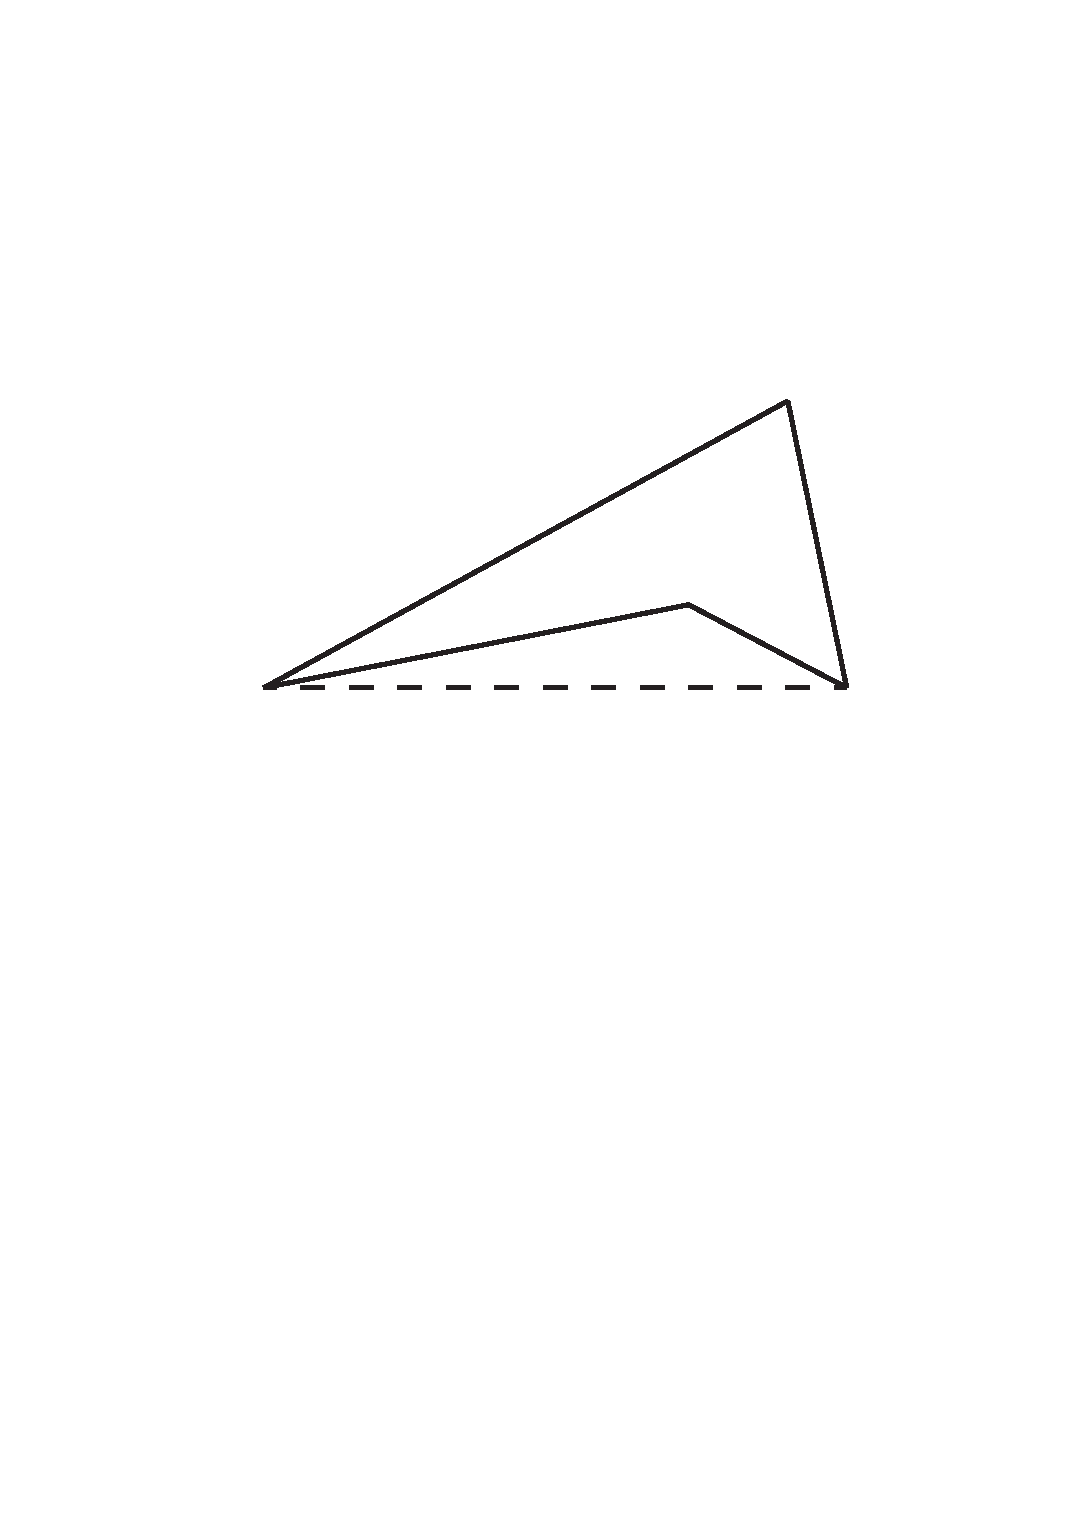
\includegraphics[width=0.9\columnwidth]{../images/geodesic_image/error_demo_triangle}\\
    \caption[Error estimation of Algorithm \ref{algorithm:app_geo}]{Error estimation of Algorithm \ref{algorithm:app_geo}, the $\overline{p_{0}p_{2}}$ is the desired geodesic while $\overline{p_{0}p_{1}}$ plus $\overline{p_{1}p_{2}}$ being the estimation.}
    \label{figure:geo_error}
\end{figure} 

Let $p_{0}$, $p_{1}$,$p_{2}$ are three points on a plane as shown in Figure \ref{figure:geo_error}. The initial path for solving Equation \ref{equation:piecewise_curvature_matrix} is $\widetilde{p_{0}p_{1}p_{2}}$ where $p_{0}$ is the source point and $p_{2}$ is the destination point. Obliviously, the true geodesic from $p_{0}$ to $p_{2}$ is $\overline{p_{0}p_{2}}$. Let $\overline{p_{0}p_{1}}$ be an established geodesic path, $p_{2}$ is an unvisited vertex. The length of edge $\overline{p_{0}p_{1}}$ is always smaller than or equals to the length of $\overline{p_{0}p_{2}}$ because the propagation only performs on outward direction. Therefore, in the worst situation, which is demonstrated in Figure \ref{figure:geo_error}, $\overline{p_{0}p_{2}}$ and $\overline{p_{0}p_{1}}$ are equal. $p'_{1}$ is the updated point calculated by Equation \ref{equation:piecewise_curvature_matrix}, Let the distance from $p'_{1}$ to edge $\overline{p_{0}p_{2}}$ is $y_{max}$, $\Vert{p_{1}p_{2}}\Vert = e$, $\Vert{p_{0}p_{1}}\Vert = \Vert{p_{0}p_{2}}\Vert = w$, $\Vert{p_{0}p'_{1}}\Vert + \Vert{p'_{1}p_{2}}\Vert = L$. Therefore, based on Heron's formula \Citep{aleksandrov1967intrinsic}, the area of $\bigtriangleup p_{0}p'_{1}p_{2}$ can be written as,
\begin{equation}
T_{\bigtriangleup p_{0}p'_{1}p_{2}} =  \frac{\sqrt{(L^{2}-w^{2})w^{2}}}{4} = \frac{wy_{max}}{2}
\end{equation}

therefore, 
\begin{equation}
L = \sqrt{4y^{2}_{max} + w^{2}}
\end{equation}

Let $err$ denotes the difference between true geodesic path length and the solution of Equation \ref{equation:piecewise_curvature_matrix}, where $err$ can be written as,

\begin{equation}
err = L - \left \| p_{0}p_{2} \right \|
= \sqrt{4y^{2}_{max} + w^{2}} - w
\end{equation}

The average error per-window over the $w$-sized window can be estimated by,

\begin{equation}
err_{ave} = \frac{\sqrt{4y^{2}_{max} + w^{2}} - w}{w}
\end{equation}

For a geodesic with $m$ sample points, the upper bound of the error is therefore estimated by,

\begin{equation}
err = m \left ( \sqrt{1 + 4(\frac{y_{max}}{w})^{2}}-1 \right ) < 2m\frac{y_{max}}{w} \sim O\left ( \varepsilon m \right )
\label{equation:geo_err}
\end{equation}

\begin{figure}[H]
	\centering
	\includegraphics[width=0.8\columnwidth]{../images/geodesic_image/cylinder_test}\\
    \caption{Error estimation of the approximate algorithm with different window size}
    \label{figure:geo_app_cylinder}
\end{figure}

where $\varepsilon=\frac{y_{max}}{w}\ll1$ and $y_{max}$ denotes the maximum offset distance of sample points to the ground truth. To have an insight into $y_{max}$, Algorithm \ref{algorithm:app_geo} is performed on a cylindrical surface, see Figure \ref{figure:geo_app_cylinder}. $\overline{p_{0}q}$ is parallel to the axis of the cylindrical surface, and the true geodesic between $p_{0}$ and $q$ is $\overline{p_{0}q}$. Let the length of the edge between each yellow point is $e$ = 1 and the window size $w$ varying from 5 to 100,  The numerical results are shown in Figure \ref{figure:geo_app_error1}. It can be noted that when $w$ = 5, the $y_{max}$ tends to be zero. But, the larger the window, the bigger the $y_{max}$. This can be explained that on the plane shown in Figure \ref{figure:geo_error}, the curvature of the geodesic estimation $\widetilde{p_{0}p_{1}p_{2}}$ is becoming smaller when window size $w$ is increased. Equation \ref{equation:piecewise_curvature_matrix} is appropriate to deal with high curvature areas. On the other hand, the window size $w$ is usually expected to be as large as possible. In Figure \ref{figure:geo_app_cylinder}, the $p_{0}$ is viewed as the start point of the window. If it is not the source, there must exist a geodesic path from source to $p_{0}$. It is ideal that the desired geodesic from source to $p_{2}$ passes through the geodesic from source to $p_{0}$. Thus, it is natural to enlarge the window size as much as possible. Figure \ref{figure:geo_app_error1} and Figure \ref{figure:geo_app_error2} shows that both the $y_{max}$ and ratio $\epsilon$ converge to small values. This means that enlarge $w$ does not reduce the error significantly. The choice of the window size $w$ should take into account the time of solving Equation \ref{equation:piecewise_curvature_matrix} rather than the computational error.

\begin{figure}[H]
        \centering
        \begin{subfigure}[b]{0.5\textwidth}
                \includegraphics[width=\textwidth]{../images/geodesic_image/app_error1}
                \caption{The convergence of $y_{max}$ with varying window size}
                \label{figure:geo_app_error1}
        \end{subfigure}%
        ~ 
        \begin{subfigure}[b]{0.5\textwidth}
                \includegraphics[width=\textwidth]{../images/geodesic_image/app_error2}
                \caption{The convergence of $\epsilon$ with varying window size}
                \label{figure:geo_app_error2}
        \end{subfigure}
        \caption{The convergenecy of error to the window size of the approximate algorithm}\label{figure:geo_app_error}
\end{figure}

In order to investigated how the running time and accuracy of Algorithm \ref{algorithm:app_geo} vary with the window size $w$ on a more complex model, MMP algorithm is performed on four character models to obtain the ground truth. The window size $w$ is varied between 5 and 100. Experimental results on four character models are reported in Figure \ref{figure:vary_window}. 


\begin{figure}[H]
        \centering
        \begin{subfigure}[b]{0.5\textwidth}
                \includegraphics[width=\textwidth]{../images/geodesic_image/absolute_error}
                \caption{Average absolute errors on four models.}
                \label{figure:window_error}
        \end{subfigure}%
        \begin{subfigure}[b]{0.5\textwidth}
                \includegraphics[width=\textwidth]{../images/geodesic_image/running_time}
                \caption{Running times on the same four models.}
                \label{figure:window_time}
        \end{subfigure}
        \caption{Performance of Algorithm \ref{algorithm:app_geo} with varying window size.}\label{figure:vary_window}
\end{figure}

According to the results, a general trend is that the approximation error decreases with an increasing window size. It drops quickly when the window size is small. However, when the window size reaches 20, the speed of improvement in accuracy starts to slow down as shown in Figure \ref{figure:window_error}. Meanwhile, the running time starts to increase more rapidly, as shown in Figure \ref{figure:window_time}. Therefore, in the character measurements extraction process, the window size $w$ is empirically set to 30.

Further to evaluate the accuracy of Algorithm \ref{algorithm:app_geo} the MMP approximation and ICH\_2 algorithms are also performed on four characters. MMP exact algorithm is performed on these four characters and its solutions are considered as the ground truth for this experiment. The absolute errors is the differences between exact geodesic distances and approximate ones and the relative errors is the ratios of absolute errors over exact distances. 

%\setlength{\tabcolsep}{4pt}
\begin{table}[H]
        %\small
        \centering
       \begin{tabular}{|m{2.1cm}|m{1.5cm}|m{1.7cm}|m{1.7cm}|m{1.7cm}|m{1.7cm}|}
        %\begin{tabular}{|c|c|c|c|c|c|}
        \hline
        \multicolumn{2}{|c|}{Characters} & A\newline\#V:127490\newline\#F:254976 & B\newline\#V:367942\newline\#F:735656 & C\newline\#V:365476\newline\#F:730760 & D\newline\#V:356544\newline\#F:712992\\
        \hline
        \multirow{2}{\columnwidth}{Algorithm \ref{algorithm:app_geo} \newline (floating)} & ave abs & 0.00309 & 0.00098 & 0.00786 & 0.005218 \\
        \cline{2-6}
                                                                    & ave rel & 0.5054\% & 0.1911\% & 1.3454\% & 0.4852\%\\
        \hline
        \multirow{2}{\columnwidth}{Algorithm \ref{algorithm:app_geo} \newline (projected)} & ave abs & 0.00401 & 0.00759 & 0.00716 & 0.01095 \\
        \cline{2-6}
                                                                        & ave rel & 1.2298\% & 1.0439\% & 1.3053\% & 1.4867\% \\
        \hline
        \multirow{2}{\columnwidth}{MMP app.} & ave abs & 0.00416 & 0.00991 & 0.00752 & 0.00917 \\
        \cline{2-6}
                                                & ave rel & 1.4183\% & 1.3665\% & 1.3283\% & 1.0886\% \\
        \hline
        \multirow{2}{\columnwidth}{ICH\_2} & ave abs & 0.00344 & 0.003751 & 0.00795 & 0.01198 \\
        \cline{2-6}
                                                & ave rel & 0.7867\% & 0.5886\% & 1.3311\% & 1.5128\% \\
        \hline
        \end{tabular}
        \caption[Error of  Algorithm \ref{algorithm:app_geo} on character models]{The average absolute and relative errors of Algorithm \ref{algorithm:app_geo}, MMP app. and ICH\_2. For Algorithm \ref{algorithm:app_geo}, $w$ = 30.}
        \label{table:tab_2} % title of Table
\end{table}


Note that, for Algorithm \ref{algorithm:app_geo}, two results are kept as one is the offset geodesics and the other is the projections of the offset geodesics onto the mesh. Table \ref{table:tab_2} gives the average absolute and average relative error of these three algorithms. 

Moreover, in order to further validate the error estimation for Algorithm \ref{algorithm:app_geo}, MMP exact algorithm is performed on the lowest resolution bunny model in Table \ref{table:fig8_tab1b} and length of the geodesics result from MMP exact algorithm is used as the ground truth. 

The ratio $\varepsilon$ in Equation \ref{equation:geo_err} is usually a very small number. Figure \ref{figure:geo_app_error3} shows the histogram of the ratio $\varepsilon$ over the bunny model, where horizontal axis indicates the value of $\varepsilon$ and vertical axis indicates the number of sample points in a geodesic. Figure \ref{figure:geo_app_error3} indicates that on the bunny model, for all geodesics, $\varepsilon$ remains a small value. 

\begin{figure}[H]
	\centering
	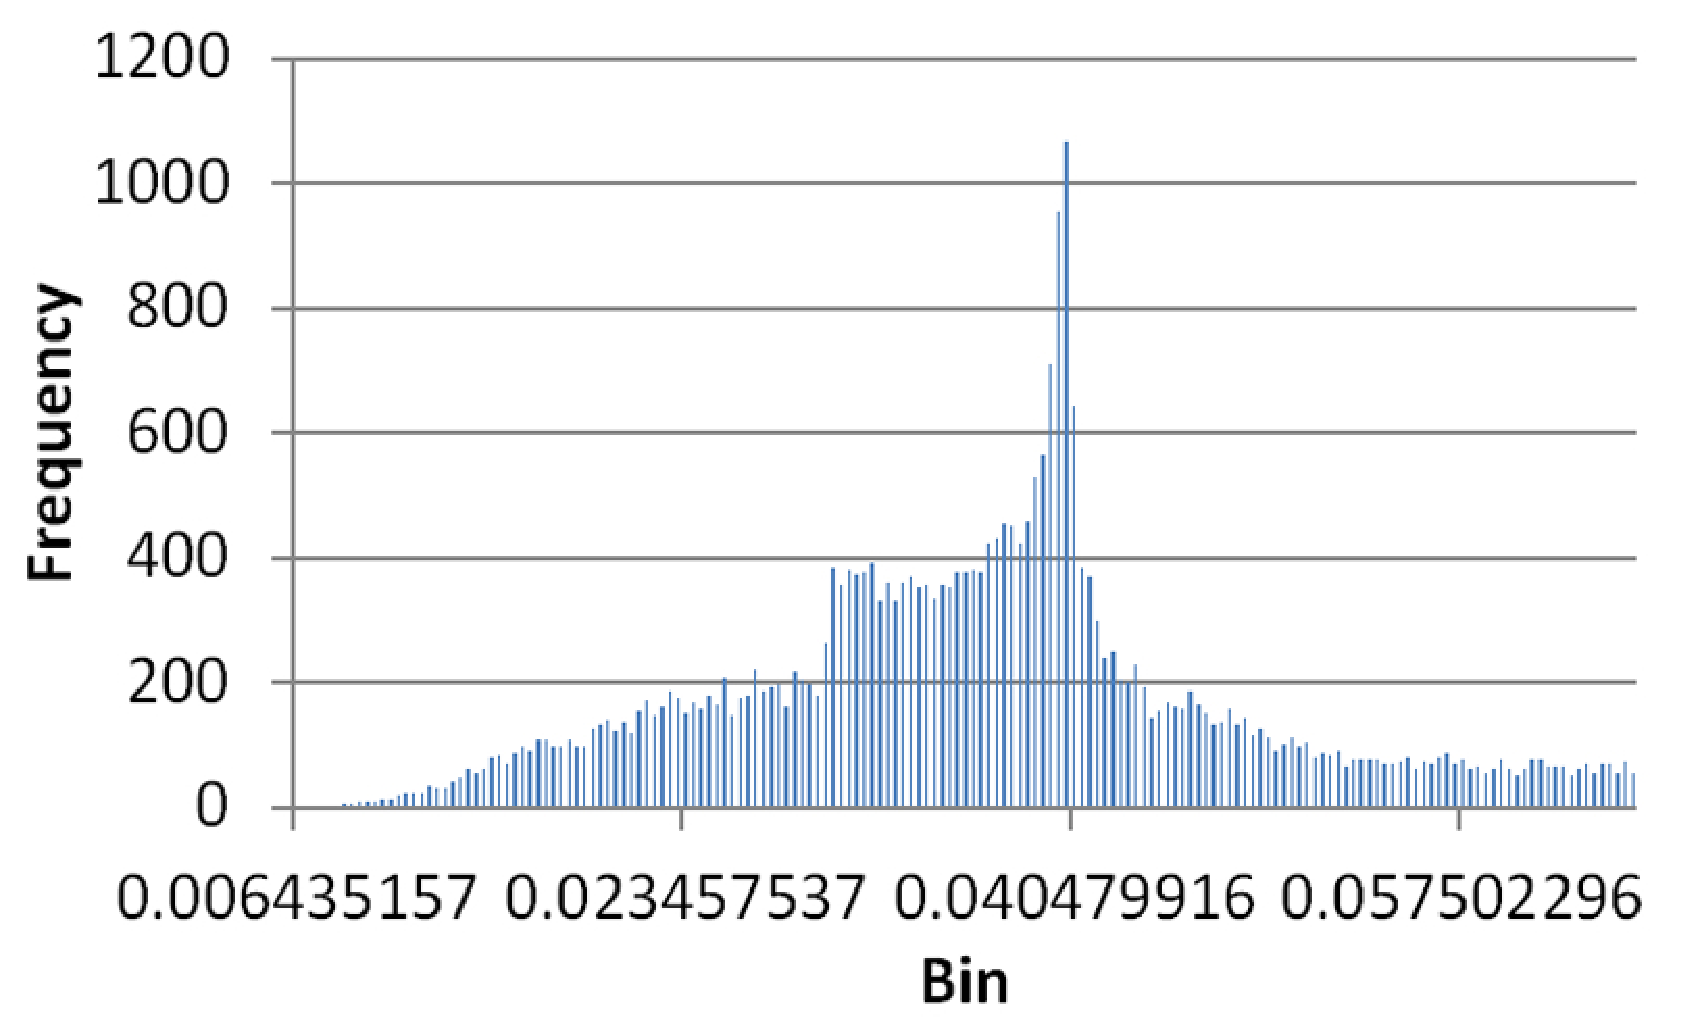
\includegraphics[width=0.9\columnwidth]{../images/geodesic_image/figure7a}\\
    \caption{Histogram of the ratio $\varepsilon$ on the bunny model}
    \label{figure:geo_app_error3}
\end{figure}

Figure \ref{figure:geo_app_error4} further shows the distribution of real absolute errors and the estimated ones in the bunny model test. It can be noted that the error estimation of Equation \ref{equation:geo_err} can accurately reflects the upper error bound of Algorithm \ref{algorithm:app_geo}



\begin{figure}[H]
	\centering	
	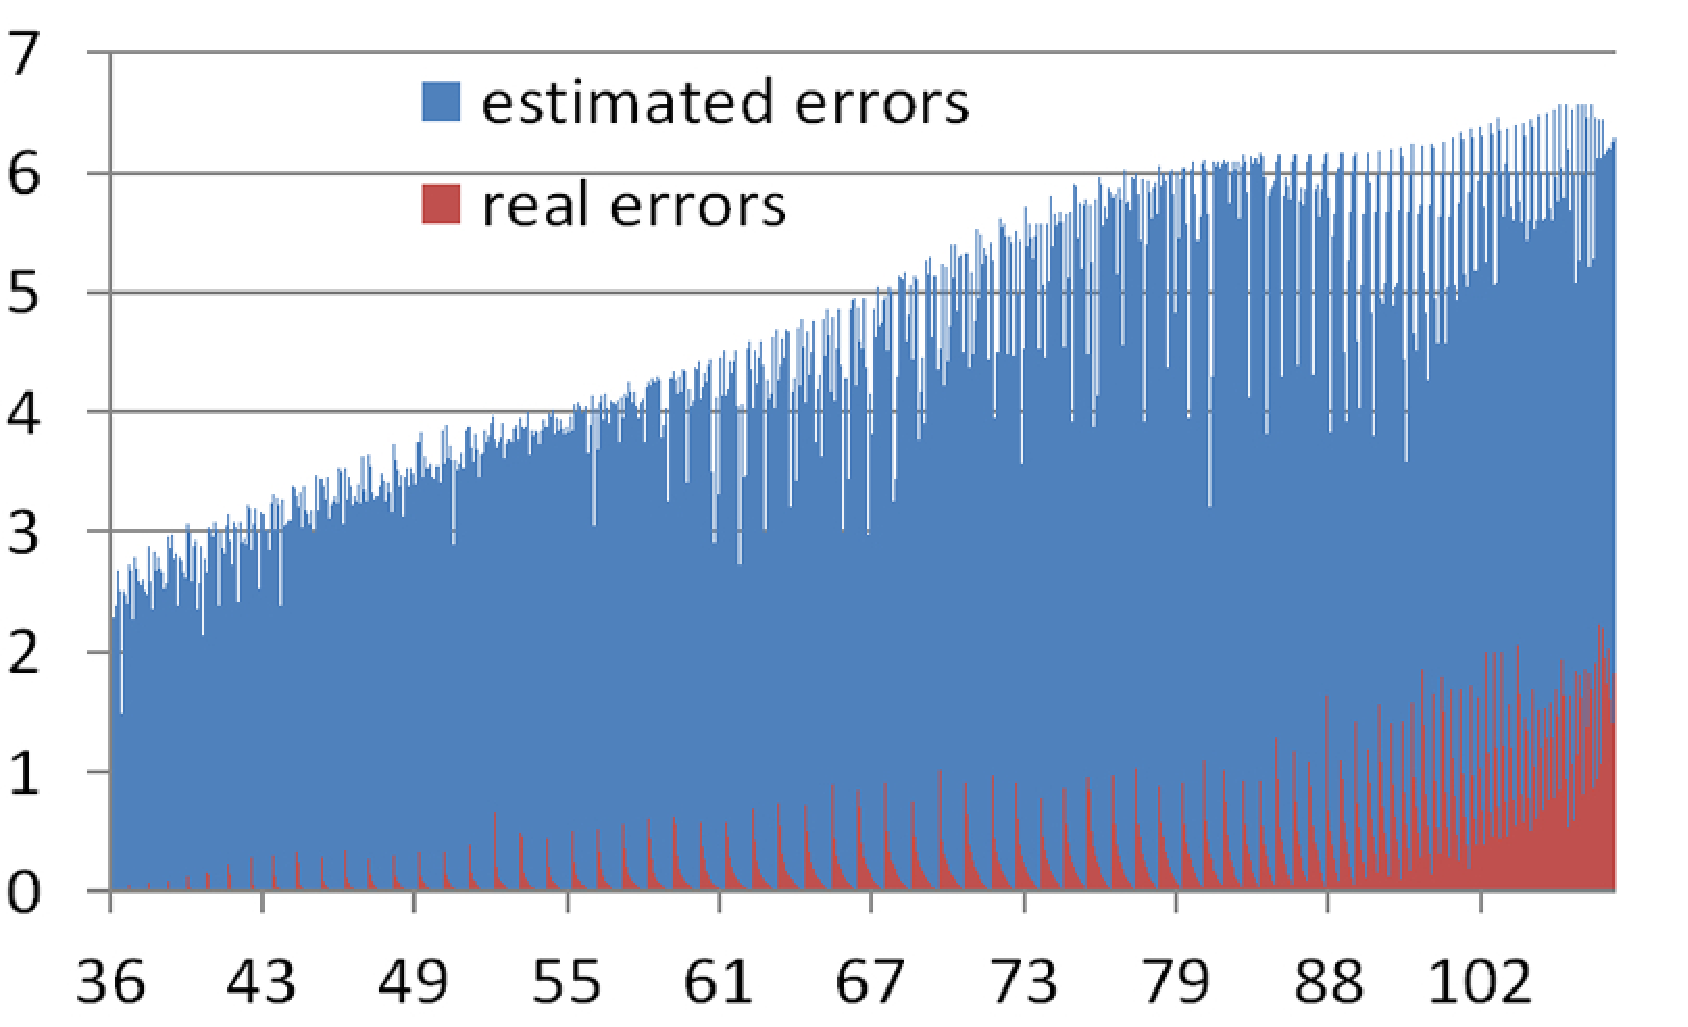
\includegraphics[width=0.9\columnwidth]{../images/geodesic_image/figure7b}\\
    \caption[The distribution of estimated errors and real errors]{The distribution of estimated errors and real errors, the window size of Algorithm \ref{algorithm:app_geo} is set to 30, the real error is bounded by the estimated error for all the geodesics on the bunny model.}
    \label{figure:geo_app_error4}
\end{figure}


%For length measurement, the geodesic algorithm presented in this chapter is applied to the character body. With each measurement, two datum points that are associated with the measurement are used as the source point and the destination point for the geodesic algorithm respectively. Figure \ref{figure:character_geodesic} demonstrates two length measurements on the character. Table \ref{table:measurements_result} lists out all the measurements used for cloth modelling in the experiment presented in the next chapter.
%
%\begin{figure}[H]
%	\includegraphics[width=\columnwidth]{../images/geodesic_on_character}\\[0.1cm]
%    \caption[Two length measurements on character]{Two length measurements on character, the ``Arm Length'' is the length of the geodesic path from ``Shoulder Point'' to ``Wrist Point'', the ``Leg Length'' is the length of the geodesic path from ``Hip Point'' to ``Outside Ankle Point'', for the datum points, see Figure \ref{figure:body_datum}.}
%    \label{figure:character_geodesic}
%\end{figure}




 

\section{Results and Conclusions}

The proposed measurement method is performed on four different characters in the same hardware environment where experiments in previous section are carried out. For length measurements extraction, Algorithm \ref{algorithm:app_geo} is utilised for geodesic path calculation. Also, MMP and ICH2 are used in order to compare the measuring efficiency. The experimental results are shown in Table \ref{table:measurements_time}.

\begin{table}[H]
    \centering
    \begin{tabular}{|p{2.5cm}|p{2cm}|p{2cm}|p{2cm}|p{2cm}|}
        \hline
        & Character A\newline\#V:127490\newline\#F:254976 & Character B\newline\#V:367942\newline\#F:735656 & Character C\newline\#V:365476\newline\#F:730760 & Character D\newline\#V:356544\newline\#F:712992\\
        
    \hline    
    Algorithm \ref{algorithm:app_geo} & 63.59s & 194.13s & 196.94s & 191.55s\\
    \hline
    MMP & 69.78s & 479.03s & 481.61s & 471.10\\
    \hline
    ICH\_2 & 65.52s & 465.19s & 466.84s & 461.91s\\
    \hline    
    \end{tabular}
    \caption{Measuring time on different characters.} % title of Table
    \label{table:measurements_time}
\end{table}

Figure \ref{figure:A_all_measurement} to \ref{figure:D_all_measurement} visualize resulting measurements on four characters. Figure \ref{figure:A_all_corrected_measurement} demonstrates length measurements with geodesic path shape correction. In these figures, red curves indicate geodesic path used for extracting length measurements, blue curves indicate convex-hull used for extracting circumference measurements. Table \ref{table:measurements_result_A} to \ref{table:measurements_result_D} lists out resulting measurement data. 
 
\begin{figure}[H]
\includegraphics[width=\textwidth]{../images/geodesic_image/A_measurement}
\caption{Measurements on Character A}
\label{figure:A_all_measurement} 
\end{figure}

\begin{figure}[H]
\includegraphics[width=\textwidth]{../images/geodesic_image/hulk_correction}
\caption{Measurements with geodesic shape correction on Character A}
\label{figure:A_all_corrected_measurement} 
\end{figure}



\begin{table}[H]
    \centering
    \begin{tabular}{|p{3.4cm}|p{1.8cm}|p{3.4cm}|p{1.8cm}|}
        \hline
        Bust Girth & 211.9015 & Sleeve length & 122.8928\\
        \hline
        Waist Girth & 73.8146 & Sleeve length\newline(with correction) & 120.1646\\
        \hline
        Hip Girth & 83.2698 & Arm hole & 157.3058\\
        \hline
        Neck Girth &67.3815 & Back length & 77.6125\\
        \hline
        Cuff Girth &59.3813 & Outside Leg length & 129.1429\\
        \hline
        Shoulder width &89.9452 & Outside Leg length\newline(with correction)& 126.2821\\
        \hline
        Back width &74.8823 & Inside Leg length & 109.7143\\
        \hline
        Front width &88.7650 & Inside Leg length\newline(with correction) & 107.2786 \\
        \hline  
        Ankle  Girth & 47.4285 & Thigh Girth & 65.5714 \\
        \hline                      
    \end{tabular}
    \caption{Measurements for characters A.} % title of Table
    \label{table:measurements_result_A}
\end{table}

  
\begin{figure}[H]
\includegraphics[width=\textwidth]{../images/geodesic_image/B_measurement}
\caption{Measurements on Character B}
\label{figure:B_all_measurement} 
\end{figure}

\begin{table}[H]
    \centering
    \begin{tabular}{|p{3.4cm}|p{1.8cm}|p{3.4cm}|p{1.8cm}|}
        \hline
        Bust Girth & 79.0833 & Sleeve length & 57.3615\\
        \hline
        Waist Girth & 70.2424 & Arm hole & 29.2281\\
        \hline
        Hip Girth & 87.2813 & Back length & 44.3503\\
        \hline
        Neck Girth &43.6637 & Outside Leg length & 89.1428\\
        \hline
        Cuff Girth &8.3771 & Inside Leg length & 74.2857\\
        \hline
        Shoulder width &40.0348 & Thigh Girth & 33.7142\\
        \hline
        Back width &38.6953 & Ankle  Girth & 16.5741\\
        \hline
        Front width &45.7562 &  &  \\
        \hline        
    \end{tabular}
    \caption{Measurements for characters B.} % title of Table
    \label{table:measurements_result_B}
\end{table}


\begin{figure}[H]
\includegraphics[width=\textwidth]{../images/geodesic_image/C_measurement}
\caption{Measurements on Character C}
\label{figure:C_all_measurement} 
\end{figure}

\begin{table}[H]
    \centering
    \begin{tabular}{|p{3.4cm}|p{1.8cm}|p{3.4cm}|p{1.8cm}|}
        \hline
        Bust Girth & 111.9165 & Sleeve length & 58.3748\\
        \hline
        Waist Girth & 96.6514 & Arm hole & 42.9157\\
        \hline
        Hip Girth & 107.5671 & Back length & 45.1839\\
        \hline
        Neck Girth &68.2416 & Outside Leg length & 85.0919\\
        \hline
        Cuff Girth &15.3368 & Inside Leg length & 71.4285\\
        \hline
        Shoulder width &51.3362 & Thigh Girth & 57.1428\\
        \hline
        Back width &50.3038 & Ankle  Girth & 20.0174\\
        \hline
        Front width &59.4946 &  &  \\
        \hline        
    \end{tabular}
    \caption{Measurements for characters C.} % title of Table
    \label{table:measurements_result_C}
\end{table}

\begin{figure}[H]
\includegraphics[width=\textwidth]{../images/geodesic_image/D_measurement}
\caption{Measurements on Character D}
\label{figure:D_all_measurement} 
\end{figure}

\begin{table}[H]
    \centering
    \begin{tabular}{|p{3.4cm}|p{1.8cm}|p{3.4cm}|p{1.8cm}|}
        \hline
        Bust Girth & 95.8160 & Sleeve length & 43.0211\\
        \hline
        Waist Girth & 70.7769 & Arm hole & 37.9510\\
        \hline
        Hip Girth & 73.1573 & Back length & 36.4173\\
        \hline
        Neck Girth &59.6871 & Outside Leg length & 51.4826\\
        \hline
        Cuff Girth &14.5720 & Inside Leg length & 41.3055\\
        \hline
        Shoulder width &34.2857 & Thigh Girth & 38.5871\\
        \hline
        Back width &32.2461 & Ankle  Girth & 21.7142\\
        \hline
        Front width &38.1302 &  &  \\
        \hline        
    \end{tabular}
    \caption{Measurements for characters D.} % title of Table
    \label{table:measurements_result_D}
\end{table}

%\begin{table}[H]
%    \centering
%    \begin{tabular}{|p{3.4cm}|p{1.8cm}|p{1.8cm}|p{1.8cm}|p{1.8cm}|}
%    %\begin{tabular}{|m{1.1cm}|m{0.8cm}|m{1.6cm}|m{1.3cm}|}
%    %\small
%    %\begin{tabular}{|c|c|c|c|c|}
%        \hline
%        & Character A & Character B & Character C & Character D\\
%        \hline
%        Bust Girth & 211.9015 & 79.0833 & 111.9165 & 95.8160\\
%        \hline
%        Waist Girth & 73.8146 & 70.2424 & 96.6514 & 70.7769\\
%        \hline
%        Hip Girth & 83.2698 & 87.2813 & 107.5671 & 73.1573\\
%        \hline
%        Neck Girth &67.3815 & 43.6637 & 68.2416 & 59.6871\\
%        \hline
%        Cuff Girth &59.3813 & 8.3771 & 15.3368 & 14.5720\\
%        \hline
%        Shoulder width &89.9452 & 40.0348 & 51.3362 & 34.2857\\
%        \hline
%        Back width &74.8823 & 38.6953 & 50.3038 & 32.2461\\
%        \hline
%        Front width &88.7650 & 45.7562 & 59.4946 & 38.1302\\
%        \hline
%        Sleeve length &122.8928 & 57.3615 & 58.3478 & 43.0211\\
%        \hline
%        Arm hole &157.3058 & 29.2281 & 42.9175 & 37.9510\\
%        \hline
%        Back length &77.6125 & 44.3503 & 45.1839 & 36.4137\\
%        \hline
%        Outside Leg length &129.1429 & 89.1428 & 85.0919 & 51.4826\\
%        \hline
%        Inside Leg length &109.7143 & 74.2857 & 71.4285 & 41.3055\\
%        \hline
%        Thigh Girth &65.5714 & 33.7142 & 57.1428 & 38.5871\\
%        \hline
%        Ankle  Girth &47.4285 & 16.5714 & 20.0174 & 21.7142\\
%        \hline        
%    \end{tabular}
%    \caption{Measurements for all the characters.} % title of Table
%    \label{table:measurements_result}
%\end{table}




The standard posture used for modelling character differs from person to person. Traditional anthropomorphic data acquisition method requires character to stay in a standard posture in order to extract the correct measurement data. Therefore, when applying traditional anthropomorphic measuring method, different character postures will result different measurements. Hence the cloth that is adjusted based on those measurements will be ill-fitted. On the contrary, geodesics are more close to the circumstance of tape measuring in the real world, it also results less variation when the posture of the character changes. 

This chapter proposed a character body measurements extraction method for animation character based on convex-hull and geodesic path computation. Calculating geodesic using current method is a time-consuming task especially on high resolution character models. In order to improve the efficiency of geodesic computation, two algorithms respectively for accurate( Algorithm \ref{algorithm:acc_geo} ) and high efficiency approximate geodesic computation( Algorithm \ref{algorithm:app_geo} ) on triangulated manifolds are proposed in this chapter. For Algorithm \ref{algorithm:app_geo}, due to the fixed window size, it is able to achieve linear time complexity with a bounded error on triangulated manifolds. Numerical comparisons with existing algorithms (i.e. MMP, ICH\_1 and ICH\_2) have further demonstrated the advantages of Algorithms \ref{algorithm:app_geo} in terms of both speed and accuracy. Experiments have shown that by integrating Algorithm \ref{algorithm:app_geo} into the measuring system, the time consumed for measuring a character has been largely reduced.


%**************************************************************************
%**************************************************************************


\ifx\isEmbedded\undefined
% References
\addcontentsline{toc}{chapter}{References}
\bibliographystyle{../ref/harvard}
\bibliography{../ref/phd_references}
\pagebreak
\end{document}
\fi
